\documentclass[11pt,a4paper]{ivoa}
\input tthdefs

\usepackage{xspace}
% Standard terms used throughout the document,
% defined as macro commands to maintain consistency
% and avoid repeated spelling mistakes.

% Using non-breaking space character.
% https://stackoverflow.com/a/1012891

\newcommand{\xml} {XML}
\newcommand{\json} {JSON}
\newcommand{\yaml} {YAML}
\newcommand{\http} {HTTP}

\newcommand{\datamodel} {data~model}
\newcommand{\webservice} {web service}
\newcommand{\webbrowser} {web browser}

\newcommand{\ivoa} {IVOA}
\newcommand{\uws} {UWS}
\newcommand{\vospace} {VOSpace}

\newcommand{\execbrokerclass} {ExecutionBroker}
\newcommand{\execworkerclass} {ExecutionWorker}
\newcommand{\executionbroker} {Execution~Broker}
\newcommand{\executionplanning} {Execution~Planning}

\newcommand{\jupyter} {Jupyter}
\newcommand{\jupyterhub} {JupyterHub}
\newcommand{\binderhub} {BinderHub}
\newcommand{\jupyternotebook} {Jupyter notebook}

\newcommand{\esap} {ESAP}
\newcommand{\escape} {ESCAPE}
\newcommand{\datalake} {DataLake}
\newcommand{\rucio} {Rucio}

\newcommand{\python} {Python}
\newcommand{\pythonprogram} {Python program}

\newcommand{\apache} {Apache}
\newcommand{\spark} {Spark}
\newcommand{\pyspark} {PySpark}
\newcommand{\zeppelin} {Zeppelin}
\newcommand{\zeppelinnotebook} {Zeppelin notebook}

\newcommand{\oci} {OCI}
\newcommand{\ociruntime} {OCI runtime}
\newcommand{\ocicontainer} {OCI container}
\newcommand{\docker} {Docker}
\newcommand{\dockercompose} {Docker compose}
\newcommand{\dockerruntime} {Docker runtime}
\newcommand{\dockercontainer} {Docker container}

\newcommand{\singularity} {Singularity}
\newcommand{\singularitycontainer} {Singularity container}

\newcommand{\openstack} {Openstack}
\newcommand{\kubernetes} {Kubernetes}

\newcommand{\codeword}[1] {\texttt{#1}}
\newcommand{\footurl}[1] {\footnote{\url{#1}}}

\newcommand{\dataset} {dataset}
\newcommand{\datascience} {data~science}
\newcommand{\scienceplatform} {science~platform}

\newcommand{\executable} {\textit{executable}}
\newcommand{\executablething} {\textit{executable}~thing}
\newcommand{\excutabletask} {\textit{executable} task}

\newcommand{\execplan} {\textit{plan}}
\newcommand{\execoffer} {\textit{offer}}
\newcommand{\workerjob} {\textit{job}}
\newcommand{\teardown} {tear-down}

\newcommand{\cpu} {CPU}
\newcommand{\gpu} {GPU}
\newcommand{\nvidiagpu} {NVIDIA~AD104~GPU}

\newcommand{\job} {\textit{job}}
\newcommand{\task} {task}

\newcommand{\scalable} {scalable}

% TODO add a citation for the YAML specification.
% https://yaml.org/spec/

\usepackage{listings}
\usepackage{xcolor}

%\colorlet{punct}{red!60!black}
\colorlet{numb}{magenta!60!black}
\definecolor{html-gray}{HTML}{EEEEEE}
\definecolor{light-gray}{gray}{0.95}
\definecolor{delim}{RGB}{20,105,176}

\lstset{
    basicstyle=\small\ttfamily,
    columns=fullflexible,
    frame=none,
    backgroundcolor=\color{light-gray},
    stepnumber=1,
    %numbers=left,
    numbers=none,
    numberstyle=\small,
    numbersep=8pt,
    %xleftmargin=\parindent,
    xrightmargin=1cm,
    showstringspaces=false,
    keepspaces=true,
    breaklines=true,
    linewidth=14cm,
    frame=none
}

% https://tex.stackexchange.com/questions/83085/how-to-improve-listings-display-of-json-files
% https://tex.stackexchange.com/a/83100
% https://tex.stackexchange.com/questions/10828/indent-a-code-listing-in-latex
% https://tex.stackexchange.com/a/10831
\lstdefinelanguage{json}{
    literate=
     *{0}{{{\color{numb}0}}}{1}
      {1}{{{\color{numb}1}}}{1}
      {2}{{{\color{numb}2}}}{1}
      {3}{{{\color{numb}3}}}{1}
      {4}{{{\color{numb}4}}}{1}
      {5}{{{\color{numb}5}}}{1}
      {6}{{{\color{numb}6}}}{1}
      {7}{{{\color{numb}7}}}{1}
      {8}{{{\color{numb}8}}}{1}
      }

\lstdefinelanguage{yaml}{
    literate=
     *{0}{{{\color{numb}0}}}{1}
      {1}{{{\color{numb}1}}}{1}
      {2}{{{\color{numb}2}}}{1}
      {3}{{{\color{numb}3}}}{1}
      {4}{{{\color{numb}4}}}{1}
      {5}{{{\color{numb}5}}}{1}
      {6}{{{\color{numb}6}}}{1}
      {7}{{{\color{numb}7}}}{1}
      {8}{{{\color{numb}8}}}{1}
      }

\hyphenation{Exe-cut-able-Thing}

\title{IVOA Execution Broker}

% see ivoatexDoc for what group names to use here; use \ivoagroup[IG] for
% interest groups.
\ivoagroup{GWS}

\author[http://www.ivoa.net/twiki/bin/view/IVOA/DaveMorris]
       {Dave Morris}
\author[http://www.ivoa.net/twiki/bin/view/IVOA/SaraBertocco]
       {Sara Bertocco}

\editor[http://www.ivoa.net/twiki/bin/view/IVOA/DaveMorris]
       {Dave Morris}

% \previousversion[????URL????]{????Concise Document Label????}
\previousversion{This is the first public release}

\begin{document}
\begin{abstract}
\label{abstract}

One of the long term goals of the IVOA has been to enable users to
move the code to the data.
This is becoming more and more important as the size and complexity
of the \dataset{}s available in the virtual observatory increases.
%\citep{gaia-at-esac}
%\footurl{https://www.skao.int/en/explore/big-data}
%\footurl{https://www.lsst.org/scientists/keynumbers}

The \ivoa{} \executionbroker{} provides a step towards making this possible.

The \ivoa{} \executionbroker{} is designed to address a specific question;
given an executable thing, e.g. a \pythonprogram{} or \jupyternotebook{}.
What facilities are available to run it?

To do this, the \ivoa{} \executionbroker{} specification defines
a \datamodel{} and \webservice{} API for describing executable things
and the resources needed to execute them.

Together these components enable a user to ask a simple question
\textit{"Where (and when) can I execute my program?"}

This in turn enables users to move code between \scienceplatform{}s.
Allowing them to develop their code on one platform and then apply it to a different
\dataset{} by sending it to execute on another platform.

\end{abstract}

\section*{Acknowledgments}
\label{acknowledgments}

The authors would like to thank all the participants in the IVOA and ESCAPE projects
who have contributed their ideas, critical reviews, and suggestions to this document.

\section*{Conformance-related definitions}

The words ``MUST'', ``SHALL'', ``SHOULD'', ``MAY'', ``RECOMMENDED'', and
``OPTIONAL'' (in upper or lower case) used in this document are to be
interpreted as described in IETF standard RFC2119 \citep{std:RFC2119}.

The \emph{Virtual Observatory (VO)} is a general term for a collection of
federated resources that can be used to conduct astronomical research,
education, and outreach.
The \href{https://www.ivoa.net}{International Virtual Observatory Alliance (IVOA)}
is a global collaboration of separately funded projects to develop standards and
infrastructure that enable VO applications.

\section{Introduction}
\label{introduction}

The \ivoa{} \executionbroker{} specification defines a \datamodel{} for describing executable tasks
and two \webservice{} interfaces, \execbrokerclass{} and \execworkerclass{}.
Together these provide a common interface for service discovery, resource allocation
and execution scheduling across a heterogeneous federation of different types of
execution platform.

\begin{itemize}
    \item \execbrokerclass{} \datamodel{}  – a data model for describing execution sessions and their resource requirements.
    \item \execbrokerclass{} \webservice{} – a discovery service to find execution platforms, allocate resources and schedule execution sessions.
    \item \execworkerclass{} \webservice{} – a monitoring service for monitoring and interacting with execution sessions.
\end{itemize}

\subsection{Role within the VO Architecture}
\label{subsec:ivoarole}

% As of ivoatex 1.2, the architecture diagram is generated by ivoatex in
% SVG; copy ivoatex/archdiag-full.xml to role_diagram.xml and throw out
% all lines not relevant to your standard.
% Notes don't generally need this.  If you don't copy role_diagram.xml,
% you must remove role_diagram.pdf from SOURCES in the Makefile.
\begin{figure}
\centering
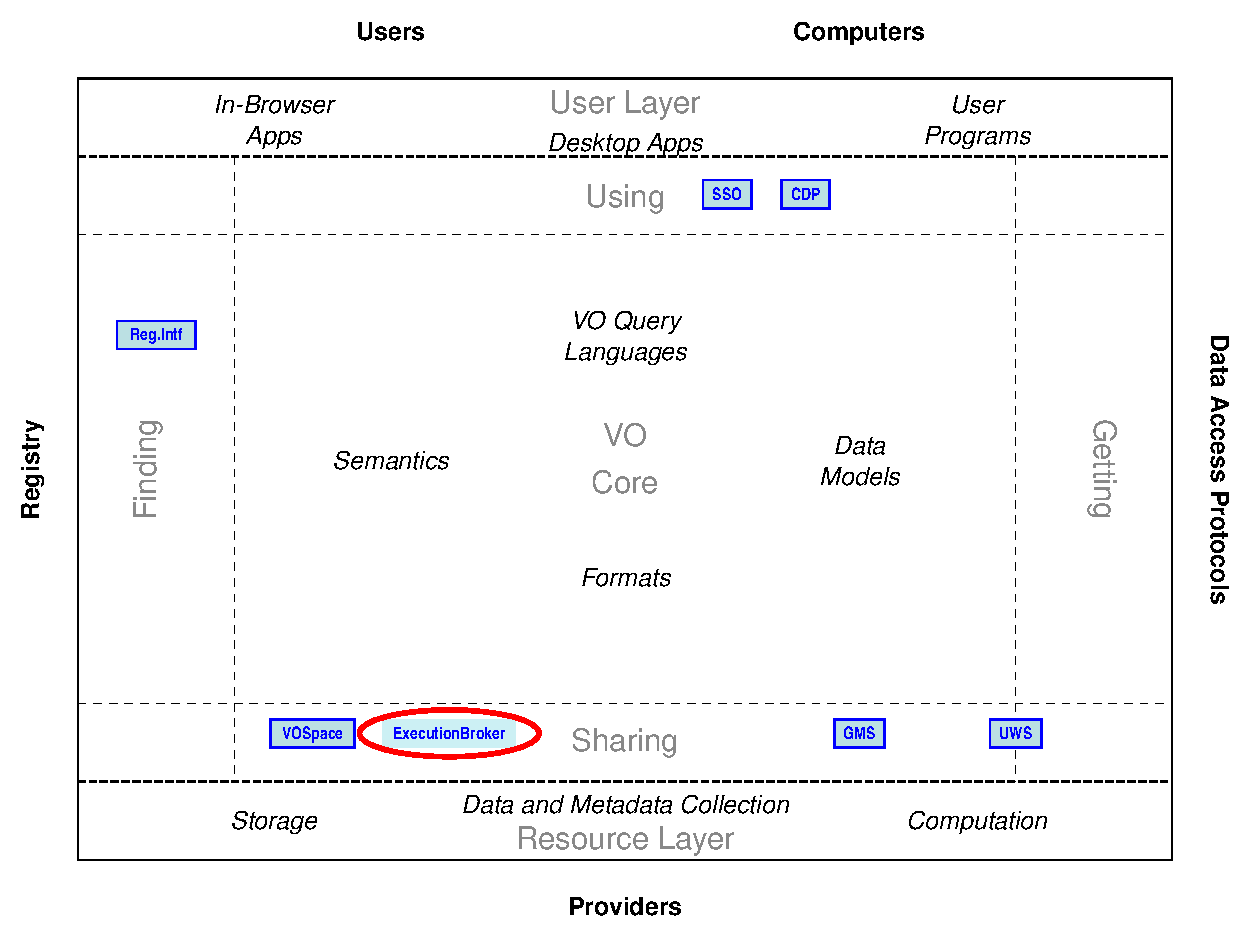
\includegraphics[width=0.9\textwidth]{role_diagram.pdf}
\caption{Architecture diagram showing the \ivoa{} \executionbroker{}'s role in the \ivoa}
\label{fig:archdiag}
\end{figure}

The IVOA Architecture\citep{2010ivoa.rept.1123A} provides a high-level view of how IVOA
standards work together to connect users and applications with providers of data
and services.
Fig.~\ref{fig:archdiag} shows the role the \ivoa{} \executionbroker{} plays within this architecture.

In response to the increasing size and complexity of the next generation of science \dataset{}s
a number of \ivoa{} members are developing intergrated \scienceplatform{}s which bring
together the \dataset{}s co-located with the compute resources needed to analyse
them.\footurl{https://data.lsst.cloud/}\footurl{https://rsp.lsst.io/index.html}

The \scienceplatform{}s make extensive use of the \ivoa{} data models and
vocabularies to describe their \dataset{}s, and use the \ivoa{} data access
services to find and access data from other data providers.
In addition, some of the \scienceplatform{}s use \ivoa{} \vospace{} services to manage
data transfers to and from local storage co-located with the compute resources.

However, to date the \ivoa{} does not provide any APIs or \webservice{} interfaces that
enable \scienceplatform{}s to exchange the software used to analyse the data.
The \ivoa{} \executionbroker{} provides a step towards making this possible.

This places the \ivoa{} \executionbroker{} in the same region of the \ivoa{} architecture
as the \ivoa{} \vospace{} specification \citep{2009ivoa.specQ1007G},
providing an infrastructure level service that enables service discovery,
resource allocation and execution scheduling across a heterogeneous federation
of execution platforms.

The \ivoa{} \executionbroker{} specification refers to the
\ivoa{} Single-Sign-On standard \citep{2017ivoa.spec.0524T}
for authentication (see section xx) %\ref{subsec:authentication}
and the
\ivoa{} Credential Delegation Protocol \citep{2010ivoa.spec.0218P}
for delegating credentials to other services.

The \ivoa{} \executionbroker{} specification also describes how to register
an \execbrokerclass{} service in the
\ivoa{} Registry \citep{2009ivoa.spec.1104B},
making it findable within the wider context of the VO.

\subsection{Executable things}
\label{executablething}

To understand the problem that the \ivoa{} \executionbroker{} is trying to solve
it is useful to describe what an \executablething{} is in this context.
In general terms, this document refers to something that can be executed, or run,
as an \executable{}.

To explain what this means we can start with a science domain function that we want to perform.
For example, the mathematical concept of the square root of a number.
We can calculate the square root of a positive number using the Newton–Raphson
algorithm\footurl{https://en.wikipedia.org/wiki/Newton\%27s_method}
which produces successively closer approximations to the result.
However, in general case, this mathematical description of the algorithm would not be
considered to be an \executablething{}.

We can write a \pythonprogram{} to use this algorithm to calculate the square root of a number.
This is the first identifiable \executablething{} in our example.
To be able to use this \executablething{}, you would need a computing resource with the appropriate
hardware and software environment. In this case, a computing resource with the \python{} interpreter
installed along with any additional \python{} modules required by the program.
This environment is often referred to as the \python{} runtime.

In the context of \scienceplatform{}s and \datascience{}, a common pattern is to provide this environment
using a Docker\footurl{https://docs.docker.com/get-started/what-is-a-container/}
or OCI\footurl{https://opencontainers.org/} container
to package the \pythonprogram{} and runtime together as a single binary object.
This package, or container, is itself an \executablething{}. One which requires a different execution
environment than the original \pythonprogram{}.
The aim of containerization is to package software components together with all the libraries and dependencies
they need as a single binary object that interfaces with a standard execution environment,
referred to as the \textit{container runtime}.
To be able to use this \executablething{}, you would need a computing resource with the appropriate
hardware and software environment. In this case, a computing resource with the \dockerruntime{} installed.

We could also create a \jupyternotebook{} that demonstrates how to use our \pythonprogram{}.
This is the third \executablething{} in our example.
One which provides an interactive environment for the user to experiment with.
As before, to be able to use this \executablething{}, we would need a computing resource with
the appropriate hardware and software environment.
In this case, a computer with the \jupyternotebook{} platform installed along with all the \python{} modules
needed by our \pythonprogram{}.
In the context of \scienceplatform{}s and \datascience{}, a common pattern is to provide this environment as a \webservice{}
that allows the user to interact with the \jupyternotebook{} via a \webbrowser.

From one algorithm that implements a science domain function, we have created three different \executablething{}s.
A \pythonprogram{}, a \dockercontainer{} packaging the \pythonprogram{}, and an interactive \jupyternotebook{}
that demonstrates how to use the \pythonprogram{}.
Each of which requires a different computing environment to execute.
A basic \python{} runtime, the \dockerruntime{}, and a \jupyternotebook{} service.

We may also want to consider the data that we are applying the algorithm to and the compute resources that
will be needed to process it.
If we are running some small experiments to learn how to use the algorithm, then a basic computing
resource will probably be sufficient.
However, if we have a \dataset{} of ten million numbers that we want to process, then we may
need to consider adding extra storage to handle the input data and the results.
For a large \dataset{} it may also be worth using a \gpu{} to accelerate the calculation steps.

The \ivoa{} \executionbroker{} \datamodel{} provides a way to describe what each of these \executablething{}s
are and what resources are needed to execute them.
This can include things like number of \cpu{} cores and amount of memory it needs,
whether it needs a \gpu{}, the location of the input data, the storage space needed to perform
the calculation and the storage space needed to save the results.

\section{Service interaction}
\label{service-interaction}

The interaction between user, client and services can be described as a conversation between the client
and one or more \execbrokerclass{} services to discover where, how, and when, an \executablething{} can be
executed.

\subsection{Discovery services}
\label{discovery-services}

The conversation starts at the discovery stage, where the user uses discovery services to
selects the software and \dataset{}s that they want to work with.

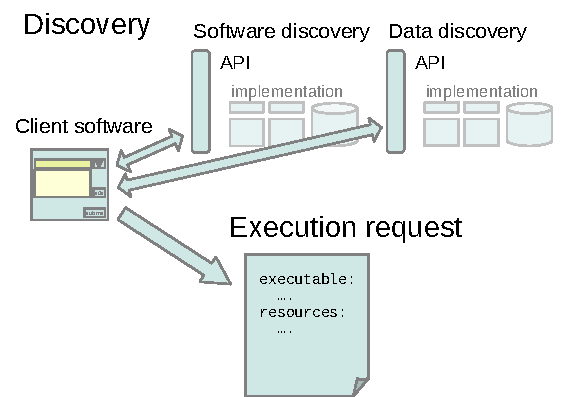
\includegraphics[width=0.9\textwidth]{diagrams/data-discovery.pdf}

The detailed specification for the software and data discovery services are beyond the
scope of this document.
However we can outline some general requirements for them.

In both cases, the discovery process should not depend on the technical details
of the software or the \dataset{}s, but on their science domain functionality and properties.

From a science user's perspective they want to be able to find software that implements
a particular clustering algorithm, or a \dataset{} that is indexed according to a particular
coordinate system.
The programming language the software is written in and the file format of the \dataset{}
are at best secondary criteria.
Ideally, if the \executionbroker{} services function as intended, a science user should not
need to know about programming languages or file formats.
The \executionbroker{} services should make all of the technical details invisible,
enabling the science user to get on with science.

The interfaces for the discovery services should be designed to be domain agnostic.
Meaning that it should be possible to swap out the astronomy based discovery services
for the equivalent biochemistry discovery services and although the domain specific
terms and vocabulary will be different, the techical details of the service interfaces
should be the same.

\subsubsection{Separation of concerns}
\label{separate-concerns}

Separate who knows what ..
The players:
\begin{itemize}
    \item The researcher who creates the notebook
    \item The developer who creates the container
    \item The publisher who publishes the data
    \item The user who is running the analysis
\end{itemize}

\subsection{Execution broker}
\label{execution-broker-desc}

Once the user has selected the \executablething{} they want to use and the
data they want to apply it to, the client combines this information to create a
description of the session the user wants to execute and sends it to one or more
\execbrokerclass{} services.
Each \execbrokerclass{} service evaluates the request and responds with a top level
\codeword{YES|NO} answer, and if
the answer is \codeword{YES}, a list of one or more offers describing how
the requested session could be executed on that platform.

%\begin{lstlisting}[]
%Request  - Can this platform execute <task> ?
%Response - YES, list of <offer>[]
%\end{lstlisting}

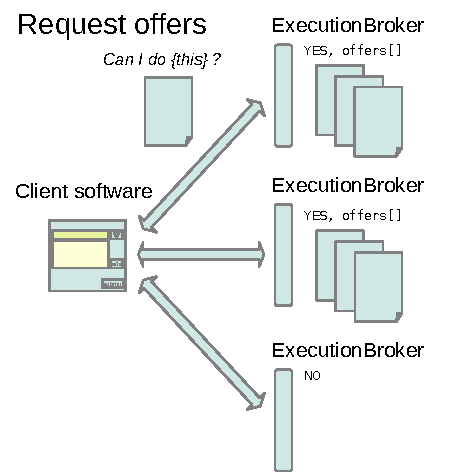
\includegraphics[width=0.9\textwidth]{diagrams/request-offers.pdf}

Each offer contains some metadata about the offer itself,
including an identifier and an expiry time,
followed by an updated version of the session description
including details of when and how it would be executed.

\begin{lstlisting}[]
# ExecutionBroker service response.
response:
  result: 'YES'
  offers:
  - ident: "f185cd47-db9b-4765-a934-bf81ee9d2d34"
    status: 'OFFERED'
    expires: "2023-09-18T07:05:21"
    body:
      executable:
        ....
      resources:
        ....
      datetime:
        ....
  - ident: "2c89f536-3fff-48f7-943f-bcc5c3225be7"
    status: 'OFFERED'
    expires: "2023-09-18T07:05:21"
    body:
      executable:
        ....
      resources:
        ....
      datetime:
        ....
\end{lstlisting}

The client can then ask its user to choose which of the offers best fits their requirements
and sends a message to the \execbrokerclass{} accepting that offer.

In response, the \execbrokerclass{} will update the status of the offer to \codeword{ACCEPTED} and return a URL
pointing to a \workerjob{} in a \execworkerclass{} service, enabling the client to monitor the \workerjob{}
status while it is executing.

%\begin{lstlisting}[]
%Request  - accept <offer>
%Response - <job details>
%\end{lstlisting}

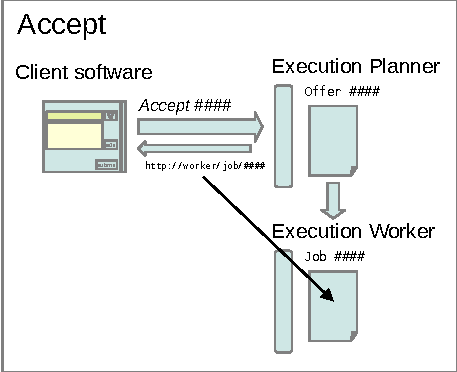
\includegraphics[width=0.9\textwidth]{diagrams/accept-offer.pdf}

Once the client has accepted an offer, the conversation between the client and the \execbrokerclass{}
is finished. Once one offer has been accepted, the \execbrokerclass{} will cancel the other offers and
release their resources.
The client does not need to cancel the offers made by the other \execbrokerclass{} services.
Offers are only valid for a limited period of time and they will expire naturally when they reach
the end of their lifetime.

How the \execbrokerclass{} and \execworkerclass{} services are linked is up to the implementation architecture.
One implementation may package both service interfaces into a single web-application.

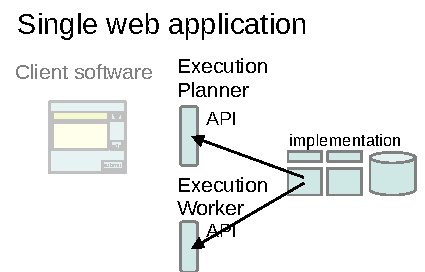
\includegraphics[width=0.9\textwidth]{diagrams/single-webapp.pdf}

Another implementation may package each of them as separate micro-services, with one \execbrokerclass{}
service providing the front-end for multiple \execworkerclass{} services.

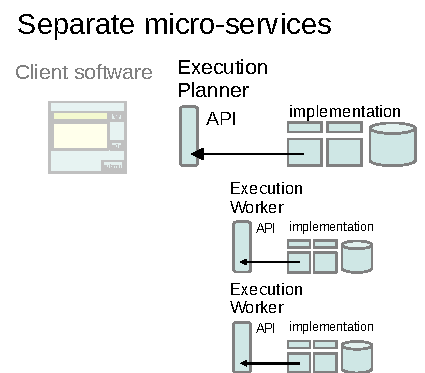
\includegraphics[width=0.9\textwidth]{diagrams/micro-services.pdf}

\subsection{Execution worker}
\label{execution-worker-desc}

The client can use the \workerjob{} details in the \execbrokerclass{} response to contact
the \execworkerclass{} service and track the \workerjob{} status.

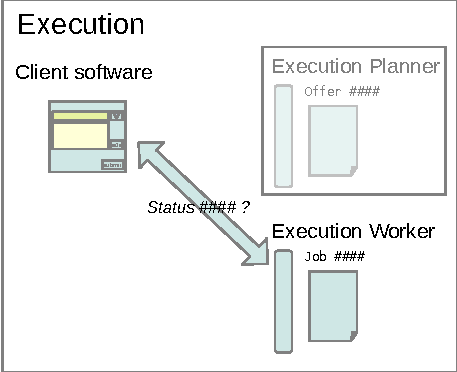
\includegraphics[width=0.9\textwidth]{diagrams/job-status.pdf}

A \workerjob{} in an \execworkerclass{} service goes through the following stages in its lifecycle.

\begin{itemize}
    \item \codeword{PENDING}   The \workerjob{} has been created, but the resources have not be prepared yet.
    \item \codeword{SETUP}     The \execworkerclass{} service is setting up the resources needed to execute the \workerjob{}.
                               This includes things like staging any \dataset{}s that will be needed locally.
    \item \codeword{READY}     The \workerjob{} is ready and waiting to start.
    \item \codeword{RUNNING}   The \workerjob{} is running.
    \item \codeword{TEARDOWN}  The execution has finished and the \execworkerclass{} service is clearing up the resources that were used.
                               This includes things like transferring the results to permanent storage and releasing local resources.
    \item \codeword{COMPLETED} The \workerjob{} has been completed.
    \item \codeword{FAILED}    The \workerjob{} failed to complete.
    \item \codeword{CANCELLED} The \workerjob{} was cancelled.
\end{itemize}

When a \execbrokerclass{} creates a \workerjob{} in an \execworkerclass{} service the
\workerjob{} starts with the \codeword{phase} set to \codeword{PENDING}.

It is up to the \execworkerclass{} to select the right time to change the \workerjob{}
\codeword{phase} to \codeword{SETUP} and start preparing the resources so that
the \workerjob{} is \codeword{READY} in time for the \codeword{starttime} declared
in the \execoffer{}.

If it will take 2 hours to transfer the input \dataset{} specified in the \execplan{}
from cold storage to live storage co-located with the compute resources,
then the \execworkerclass{} needs to start the \codeword{SETUP} phase at least 2 hours
before the \codeword{starttime} declared in the \execoffer{}.

Once all the resources are ready, the \execworkerclass{} changes the \workerjob{}
\codeword{phase} to \codeword{READY} to indicate that the all the resources
are ready and the \workerjob{} is waiting to start.

For a normal \execplan{} with no triggers, the \workerjob{} will be started at
the \codeword{starttime} declared in the \execoffer{}.

For an \execplan{} with a start trigger, the \workerjob{} will stay at \codeword{phase}
\codeword{READY} until the start trigger is received.

When the \workerjob{} start executing, the \codeword{phase} is changed to \codeword{RUNNING}
to indicate that the \workerjob{} is running.

When the \workerjob{} finishes executing, because the \dockercontainer{} finished executing,
the user closed their \jupyternotebook, or the \codeword{maxduration} was reached,
the \execworkerclass{} will change the \workerjob{} \codeword{phase} to \codeword{TEARDOWN} and
begin the process of releasing the resources.

If the \execplan{} declared some persistent storage that will last beyond the end of the \workerjob{},
then part of the \teardown{} process may involve transferring results from the \workerjob{}
onto the persistent storage before the local storage is released.

When the \teardown{} process completes, the \workerjob{} \codeword{phase} is changed to \codeword{COMPLETED}.

If an error occurs at any time in the process, the \workerjob{} \codeword{phase} is changed to \codeword{FAILED}.
This includes any errors that occur during the \teardown{} process; for example, because
the \execworkerclass{} was unable to transfer the results onto persistent storage.
Then the \workerjob{} \codeword{phase} is changed to \codeword{FAILED}, even if the main part of the
execution completed successfully.
This is because any workflow steps that follow after this step, will depend not only on the execution being
completed, but they also need the \teardown{} data transfers to complete so that the results from this step
are in the right place for the next step to be able to access them.

\section{The \executable{}}
\label{executable}

At the simplest level the client just needs to check whether a platform is able to execute a particular
type of \excutabletask{}.
For example, \textit{"Is this platform able to run a \jupyternotebook{}?"}

In order to do this, the request needs to specify the task type, e.g. \jupyternotebook{},
along with details about it, e.g. where to fetch the notebook from.

The information in this part of the \datamodel{} will be different for each type of \executable{}.
Rather than try to model every possible type of \executable{} in one large \datamodel{},
the \datamodel{} for each type is described in an extension to the core \datamodel{}.

To support this, the core \datamodel{} defines two fields:
\begin{itemize}
  \item \codeword{type} - a URI identifying the type of \executable{}.
  \item \codeword{spec} - a place holder for type specific details.
\end{itemize}

% Type URLs
% https://www.purl.org/ivoa.net/executable-types/example
% https://github.com/ivoa-std/ExecutionBroker/blob/main/types/executable-types/example-executable.md
\begin{lstlisting}[]
# ExecutionBroker client request.
request:
  # Details of the executable.
  executable:

    # A URI identifying the type of executable.
    type: "https://www.purl.org/ivoa.net/executable-types/example"

    # The details, specific to the type of executable.
    spec: {}
\end{lstlisting}

\subsection{\jupyternotebook{}}
\label{jupyternotebook}
The \datamodel{} for each type of \executable{} defines the metadata needed to
describe that particular type.
For example, the \datamodel{} for a \jupyternotebook{} needs to describe where
to fetch the source code for the notebook from.

% Type URLs
% https://www.purl.org/ivoa.net/executable-types/jupyter-notebook
% https://github.com/ivoa-std/ExecutionBroker/blob/main/types/executable-types/jupyter-notebook.md
\begin{lstlisting}[]
# ExecutionBroker client request.
request:
  # Details of the executable.
  executable:
    # A URI identifying the type of executable.
    type: "https://www.purl.org/ivoa.net/executable-types/jupyter-notebook"

    # The details, specific to a Jupyter notebook.
    spec:
      notebook: "https://.../example.jpnb"
\end{lstlisting}

It may also include a reference to a \codeword{requirements.txt} file that describes any additional \python{}
libraries needed to run the notebook.
\begin{lstlisting}[]
# ExecutionBroker client request.
request:
  # Details of the executable.
  executable:
    # A URI identifying the type of executable.
    type: "https://www.purl.org/ivoa.net/executable-types/jupyter-notebook"

    # The details, specific to a Jupyter notebook.
    spec:
      notebook: "https://.../example.jpnb"
      requirements: "https://.../requirements.txt"
\end{lstlisting}

\subsection{\dockercontainer{}}
\label{dockercontainer}
The \datamodel{} for an \dockercontainer{} describes the image name and version
along with the hostname of the repository to fetch it from.

% Type URLs
% https://www.purl.org/ivoa.net/executable-types/oci-container
% https://github.com/ivoa-std/ExecutionBroker/blob/main/types/executable-types/oci-container.md
\begin{lstlisting}[]
# ExecutionBroker client request.
request:
  # Details of the executable.
  executable:
    # A URI identifying the type of executable.
    type: "https://www.purl.org/ivoa.net/executable-types/docker-container"

    # The details, specific to a Docker container.
    spec:
      repo:  "ghcr.io"
      image: "ivoa/oligia-webtop"
      version: "ubuntu-2022.01.13"
\end{lstlisting}

This pattern of using a \codeword{type} URI to identify the type of thing, and then a
\codeword{spec} block to add the type specific details is used in several places in the
\executionbroker{} \datamodel{}.
This enables us to keep the core \datamodel{} relatively small, defining the common aspects
needed to describe an \executablething{} and the resources it needs while allowing the
\datamodel{} to be extended to describe a wide range of different types of things.

This pattern makes it easy for projects outside the core \ivoa{} community to add new
types of \executablething{}s and resources appropriate for their science domain.

Using a URI to identify the task type means that implementations do not need to understand
all of the different possible types of \executable{}.
If a service doesn’t recognize a particular type, it can simply reply \codeword{NO}.

\begin{lstlisting}[]
Request  - Can this platform execute <unkown-type> ?
Response - NO
\end{lstlisting}

\section{Resources}
\label{resources}

At the next level the client may need to check whether a platform has sufficient compute resources
needed to execute a particular task.
For example, \textit{"Can this platform provide enough resources to run this \jupyternotebook{}?"}

In order to do this the request would not only need to describe the \executable{} itself,
but also the minimum level of compute resources needed in terms of \cpu{} cores, memory, \gpu{}s
and disc space needed to execute it.

\subsection{Compute resources}
\label{compute-resources}

The \datamodel{} for describing compute resources is, in most cases, common to all types of \executable{},
so the \datamodel{} for these requirements are defined as part of the core \executionbroker{} \datamodel{}.

It is important to note that all of the resource requirements are optional.
As in the example from the previous section, a request to execute a simple \jupyternotebook{}
does not need to include any resource details.

\begin{lstlisting}[]
# ExecutionBroker client request.
request:
  # Details of the executable.
  executable:
    # A URI identifying the type of executable.
    type: "https://www.purl.org/ivoa.net/executable-types/jupyter-notebook"

    # The details, specific to a Jupyter notebook.
    spec:
      notebook: "https://.../example.jpnb"
\end{lstlisting}

As long as this \jupyternotebook{} only needs a minimal set of resources to run, e.g.
2 \cpu{} cores, 2G of memory and 20G of disc space, then this task probably doesn't need
any additional resources.

However, if this \jupyternotebook{} needs a specific type of \gpu{} to function properly,
then it can be added to the request by specifying a compute resource with the specific type
of \gpu{}.

% Type URLs
% https://www.purl.org/ivoa.net/resource-types/generic-compute
% https://github.com/ivoa-std/ExecutionBroker/blob/main/types/resource-types/generic-compute.md
% Type URLs
% https://tinyurl.com/nvidia-ad104
% https://www.purl.org/ivoa.net/resource-types/nvidia-ad104
% https://github.com/ivoa-std/ExecutionBroker/blob/main/types/resource-types/nvidia-ad104.md
\begin{lstlisting}[]
# ExecutionBroker client request.
request:
  # Details of the executable.
  executable:
    # A URI identifying the type of executable.
    type: "https://www.purl.org/ivoa.net/executable-types/jupyter-notebook"
    # The details, specific to a Jupyter notebook.
    spec:
      notebook: "https://.../example.jpnb"

  # Details of the resources needed.
  resources:
    compute:
    - name: "compute-001"
      type: "https://www.purl.org/ivoa.net/resource-types/generic-compute"
      spec:
        extras:
        - name: "nvidia-gpu"
          # A URI identifying the type of GPU.
          type: "https://tinyurl.com/nvidia-ad104"
\end{lstlisting}

With this detail added to the request, platforms that are not able to provide this kind of \gpu{}
would simply reply \codeword{NO}.

\begin{lstlisting}[]
Request  - Can this platform provide 'NVIDIA AD104 GPU' ?
Response - NO
\end{lstlisting}

Note that a platform does not need to know what a  "\nvidiagpu{}" is to be able to reply with a sensible aswer.
If a platform receives a request for a resource that it doesn't understand, it MAY simply reply \codeword{NO}.

\begin{lstlisting}[]
Request  - Can this platform provide <unknown extra> ?
Response - NO
\end{lstlisting}

The only platforms that will reply \codeword{YES} are ones that understand what a "\nvidiagpu{}"
is and are able to provide access to one.

The \datamodel{} for the \gpu{} resource follows the same extendable pattern as the \datamodel{} for
the \executable{}. A \codeword{type} URI to identify the type of \gpu{},
and a \codeword{spec} section for type specific details,
e.g. the minimum amount of memory and number of shaders.

% Type URLs
% https://tinyurl.com/nvidia-ad104
% https://www.purl.org/ivoa.net/resource-types/nvidia-ad104
% https://github.com/ivoa-std/ExecutionBroker/blob/main/types/resource-types/nvidia-ad104.md
\begin{lstlisting}[]
# ExecutionBroker client request.
request:
  # Details of the executable.
  executable:
    ....
  # Details of the resources needed.
  resources:
    compute:
    - name: "compute-001"
      type: "https://www.purl.org/ivoa.net/resource-types/generic-compute"
      spec:
        extras:
        - name: "nvidia-gpu"
          # A URI identifying the type.
          type: "https://tinyurl.com/nvidia-ad104"
          # The details, specific to a 'NVIDIA AD104 GPU'.
          spec:
            minmemory: 20
            minshaders: 6144
\end{lstlisting}

This pattern make it easy for projects to add new types of compute resources to their
platforms. All they need to do is to choose a URL to identify the \codeword{type}
and they can add their own type specific details to the \codeword{spec} section.

% Type URLs
% https://tinyurl.com/xilinx-vu19p
% https://www.purl.org/ivoa.net/resource-types/xilinx-vu19p
% https://github.com/ivoa-std/ExecutionBroker/blob/main/types/resource-types/xilinx-vu19p.md
\begin{lstlisting}[]
# ExecutionBroker client request.
request:
  # Details of the executable.
  executable:
    ....
  # Details of the resources needed.
  resources:
    compute:
    - name: "compute-001"
      type: "https://www.purl.org/ivoa.net/resource-types/generic-compute"
      spec:
        extras:
        - name: "Xilinx FPGA"
          # A URI identifying the type.
          type: "https://www.purl.org/ivoa.net/resource-types/xilinx-vu19p"
          # The details, specific to a 'Xilinx FPGA'.
          spec:
            logicCells: 8938
            DSPslices:  3840
\end{lstlisting}

Note that in both these examples, the URL used to identify the \codeword{type}
uses some level of indirection to make the URL more robust.

At the time of writing, the best resource we could find to describe NVIDIA's AD104 GPU
is an entry in a database curated by the TECHPOWERUP
website\footurl{https://www.techpowerup.com/gpu-specs/nvidia-ad104.g1013}.
While this page provides a lot of useful techical detail about the component,
the URL itself is vulnerable to changes in the design of the TECHPOWERUP website.

To make this more robust we can use a URL redirect service to create a more permanent
URL that we have control over\footurl{https://tinyurl.com/nvidia-ad104}.
If the TECHPOWERUP website is redesigned, we can update
our redirect to match.

There are several options to choose from:
\begin{itemize}
\item A URL shortening service.\\
      \codeword{[https://tinyurl.com/nvidia-ad104]}
\item The PURL service\footurl{https://purl.archive.org/} provided by the internet archive\footurl{http://www.archive.org/}.\\
      \codeword{[https://www.purl.org/ivoa.net/resource-types/nvidia-ad104]}.
\item A page in our GitHub repository that directs the reader to more resources\footurl{https://github.com/ivoa-std/ExecutionBroker/blob/main/types/resource-types/nvidia-ad104.md}.\\
      \codeword{[https://github.com/..../resource-types/nvidia-ad104.md]}.
\end{itemize}

Similarly, the best resource we could find to decribe the Xilinx FPGA provided by Amazon AWS
F1\footurl{https://aws.amazon.com/ec2/instance-types/f1/} instances is the product details
page on the Xilinx website\footurl{https://www.xilinx.com/products/silicon-devices/fpga/virtex-ultrascale-plus-vu19p.html}.
Both of these URLs are informative, but are vulnerable to changes in their websites.

To make this more robust, our example uses a PURL redirect to a page in our GitHub repository that describes
the type of FPGA that our project requires. The page in our GitHub repository can point to additional details about the
FPGA and the tools needed to use it.
\begin{itemize}
%\item A URL shortening service \codeword{[https://tinyurl.com/xilinx-vu19p]}.
\item A PURL redirect to provide a long lasting URL.\\
      \codeword{[https://www.purl.org/ivoa.net/resource-types/xilinx-vu19p]}
\item A page in our GitHub repository describing the FPGA and the tools needed to use it\footurl{https://github.com/ivoa-std/ExecutionBroker/blob/main/types/resource-types/xilinx-vu19p.md}.\\
      \codeword{[https://github.com/..../resource-types/xilinx-vu19p.md]}
\end{itemize}

\subsection{Minimum and maximum}
\label{minandmax}

The \datamodel{} for describing compute resources includes elements for specifying the numeric size
and number of resources such as \cpu{} cores, memory and storage.

If the \jupyternotebook{} in our example needs a minimum of 8 \cpu{} cores and 16G of memory
to be able to perform its calculations, then this can be specified in the compute resource.

\begin{lstlisting}[]
# ExecutionBroker client request.
request:
  # Details of the executable.
  executable:
    ....
  # Details of the resources needed.
  resources:
    compute:
    - name: "compute-001"
      type: "https://www.purl.org/ivoa.net/resource-types/generic-compute"
      spec:
        mincores:   8
        minmemory: 16
\end{lstlisting}

All of the \datamodel{} elements for specifying the size or number of resources are defined
as pairs of minimum and maximum values.
This allows a conversation between the \execbrokerclass{} client and services
to discover the best platform to execute the task.

The client requests the minimun resources it needs,
and each service responds with a set of offers which specify the maximum
level of resources they can offer.

For example, if a platform is able to provide double the compute resources,
16 \cpu{} cores and 32G of memory,
then it can indicate this by specifying higher maximum values in its response.

\begin{lstlisting}[]
# ExecutionBroker service response.
response:
  # Details of the executable.
  executable:
    ....
  # Details of the resources offered.
  resources:
    compute:
    - name: "compute-001"
      type: "https://www.purl.org/ivoa.net/resource-types/generic-compute"
      spec:
        mincores:   8
        maxcores:  16
        minmemory: 16
        maxmemory: 32
\end{lstlisting}

This response represents an offer to start with a minimum of 8 \cpu{} cores and 16G of memory
as requested, with the option to use a maximum of 16 \cpu{} cores and 32G of memory if needed.

The client may receive different offers from different platforms and can pass this information
on the user to allow them to choose the offer that best fits their use case.
The notebook they have chose may specify a minimum of 8 \cpu{} cores and 16G of memory,
but an offer of twice the resources allows the user more scope for experimenting with
more data or more complex algorithms.

This \scalable{} compute resource represents something like a \kubernetes{} platform where the
execution can start with a minimum configuration and scale on demand up to a maximum limit.

This is slightly different to a platform like \openstack{} which allocates resources
in specific blocks, defined by the set of \textit{'flavors'} available on that particular platform.
If the smallest flavor of virtual machine available on the platform has 16 \cpu{} cores and 24G of memory,
then the service can represent that by setting the minimum values in its offer to match available resources.

\begin{lstlisting}[]
# ExecutionBroker service response.
response:
  # Details of the executable.
  executable:
    ....
  # Details of the resources offered.
  resources:
    compute:
    - name: "compute-001"
      type: "https://www.purl.org/ivoa.net/resource-types/generic-compute"
      spec:
        mincores:  16
        maxcores:  16
        minmemory: 24
        maxmemory: 24
\end{lstlisting}

This response represents an offer to start with a fixed allocation of 16 \cpu{} cores and 24G of memory.

An \execbrokerclass{} MAY NOT make an offer with less than the minimum resources requested.
For example, if an \openstack{} platform only has a virtual machine flavor with 1 \cpu{} core and 2G of memory,
then it MAY NOT offer this resource as it is less than the requested minimum.

Note that the term \textit{'compute resource'} specifically avoids stating whether the
notebook will be run in an \openstack{} virtual machine or a \kubernetes{} cluster.
As far as the user is concerned, it should not matter. As long as the compute resource provides
sufficient \cpu{} cores and memory for the notebook to execute, the technical details of how the
platform implements this should not be relevant at this level of abstraction.

The user just wants their notebook to run. The technical details of what technologies are used
under the hood to make it happen should be someone else's problem.

\subsection{Storage resources}
\label{storage-resources}

The resources section of the request can also be used to specify storage resources.

There are two main types of storage resources:
\begin{itemize}
    \item Internal storage resources that are provided by the platform.
    \item External storage resources that are provided by an external source.
\end{itemize}

There are two types of internal storage resources:
\begin{itemize}
    \item Ephemeral storage available for the duration of the \job{}, created when the \job{} starts and released when the \job{} is completed.
    \item Persistent storage that exists beyond the lifetime of the \job{}, created before the \job{} starts and remaining after the \job{} has completed.
\end{itemize}

There are two levels of persistent storage:
\begin{itemize}
    \item Managed resources that are created and deleted by the platform.
    \item Unmanaged resources that are created and deleted by an external entity.
\end{itemize}

The simplest of these are ephemeral storage resources managed by the execution platform.
For example, if the \jupyternotebook{} in our example requires 1024GiB of space to perform its calculations,
then this can be specified in the request by defining an ephemeral storage resource.

% Type URLs
% https://www.purl.org/ivoa.net/storage-types/ephemeral-storage
% https://github.com/ivoa-std/ExecutionBroker/blob/main/types/storage-types/ephemeral-storage.md
\begin{lstlisting}[]
# ExecutionBroker client request.
request:
  # Details of the executable.
  executable:
    ....
  # Details of the resources needed.
  resources:
    ....
    storage:
    - name: "scratch-space"
      type: "https://www.purl.org/ivoa.net/storage-types/ephemeral-storage"
      spec:
        size: 1024
\end{lstlisting}

To enable the \jupyternotebook{} to access this storage, we need to add a
corresponding \codeword{volume} element to the compute resource that describes
where to mount the storage resource.

For example, the following request asks for 1024GiB of ephemeral storage
that is mounted at \codeword{/temp} in the filesystem of the compute resource.
The compute volume is linked to the storage resource by the name of the
storage resource.

\begin{lstlisting}[]
# ExecutionBroker client request.
request:
  # Details of the executable.
  executable:
    ....
  # Details of the resources needed.
  resources:
    ....
    compute:
    - name: "compute-001"
      ....
      volumes:
      - name: "temp-volume"
        resource: "scratch-space"
        path: "/temp"
        mode: "rw"
    storage:
    - name: "scratch-space"
      type: "https://www.purl.org/ivoa.net/storage-types/ephemeral-storage"
      spec:
        size: 1024
\end{lstlisting}

This pattern of separating the details of how a storage resource is implemented
from the details of how it is mounted inside a computing resource is based on a
pattern used by \kubernetes{} to describe storage volumes and their mount points
within containers\footurl{https://kubernetes.io/docs/concepts/storage/volumes/}.

This pattern can also be used to define a storage resource that imports data from
an external source.
For example, if the user wanted to use the \jupyternotebook{} to analyse data stored
in an external S3 system, this can be done by defining an external storage resource
that describes where the data is,
and a corresponding volume mount inside the compute resource.

% Type URLs
% https://www.purl.org/ivoa.net/storage-types/amazon-s3
% https://github.com/ivoa-std/ExecutionBroker/blob/main/types/storage-types/amazon-s3.md
\begin{lstlisting}[]
# ExecutionBroker client request.
request:
  # Details of the executable.
  executable:
    ....
  # Details of the resources needed.
  resources:
    ....
    compute:
    - name: "compute-001"
      ....
      volumes:
      - name: "data-volume"
        resource: "source-data"
        path: "/data"
        mode: "r"
    storage:
    - name: "source-data"
      type: "https://www.purl.org/ivoa.net/storage-types/amazon-s3"
      spec:
        endpoint: "https://.../echo"
        bucket: "example-data"
\end{lstlisting}

Again, this pattern of separating how the data is stored outside the system
and how it appears inside the compute resource borrows heavily from the
pattern used by \kubernetes{} to describe persistent
volumes\footurl{https://kubernetes.io/docs/concepts/storage/persistent-volumes/}.

The same pattern can be used to describe a storage resource that can be used
to save the analysis results, by defining a persistent storage resource
allocated by the system, and a corresponding volume mount inside the compute resource.

% Type URLs
% https://www.purl.org/ivoa.net/storage-types/persistent-storage
% https://github.com/ivoa-std/ExecutionBroker/blob/main/types/storage-types/persistent-storage.md
\begin{lstlisting}[]
# ExecutionBroker client request.
request:
  # Details of the executable.
  executable:
    ....
  # Details of the resources needed.
  resources:
    ....
    compute:
    - name: "compute-001"
      ....
      volumes:
      - name: "results-volume"
        resource: "results-storage"
        path: "/results"
        mode: "rw"
    storage:
    - name: "results-storage"
      type: "https://www.purl.org/ivoa.net/storage-types/persistent-storage"
      spec:
        lifecycle: "managed"
        minlifetime: "1D"
        minsize: 100
\end{lstlisting}

By setting the storage resource type to \codeword{https://.../persistent},
and setting the \codeword{lifecycle} to \codeword{managed},
the client is asking the \execbrokerclass{} service to take care of allocating
the storage and managing its lifecycle.
It is up to the \execbrokerclass{} service to decide where to store the data and
how make it accessible after the \job{} has completed.

For example, a science platform may have a \rucio{} storage system co-located
with the compute platform which it uses to store user generated data.
In which case the \execbrokerclass{} service would respond with an offer that
stores the results in the \rucio{} system and provides details of how the user
can access it after the \job{} has completed.

% Type URLs
% https://www.purl.org/ivoa.net/storage-types/rucio-storage
% https://github.com/ivoa-std/ExecutionBroker/blob/main/types/storage-types/rucio-storage.md
\begin{lstlisting}[]
# ExecutionBroker service response.
response:
  # Details of the executable.
  executable:
    ....
  # Details of the resources offered.
  resources:
    ....
    compute:
    - name: "compute-001"
      ....
      volumes:
      - name: "results-volume"
        resource: "results-storage"
        path: "/results"
        mode: "rw"
    storage:
    - name: "results-storage"
      type: "https://www.purl.org/ivoa.net/storage-types/rucio-storage"
      spec:
        lifecycle: "managed"
        minlifetime: "1D"
        maxlifetime: "5D"
        minsize:  100
        maxsize:  200
        endpoint: "http://...."
        domain: "Project 51"
        objectid: "cdc78e7d-8032-497e-9a5b-01c720ea2223"
\end{lstlisting}

In this example, the client requested at least 100G of storage available for 1 day
and in response the service is offering up to 220G available for 5 days stored in a
\rucio{} system co-located close to the compute platform.
It is up to the client to check if it can access the particular \rucio{} system
described in the response before it accepts the offer.

Making an offer with the \codeword{lifecycle} set to \codeword{managed} and the
\codeword{maxlifetime} set to \codeword{5D}
means that the service will manage the lifecycle.
The storage will be available for 5 days after the \job{} completes and then it
will be deleted automatically.
The client doesn't need to worry about tidying up afterwards.

It is important to note that at this point in time the storage is proposed, but not yet allocated.
The persistent storage is only allocated if the client accepts this particular offer.
This allows an \execbrokerclass{} service to make multiple offers with different storage options,
allowing the client to select and accept the one that best fits its use case.

The same \datamodel{} can be used the other way around as well.
If the client already knows where it wants the data to be stored, for example at a specific
\vospace{} location, then it can specify this in the request.

% Type URLs
% https://www.purl.org/ivoa.net/storage-types/vospace-storage
% https://github.com/ivoa-std/ExecutionBroker/blob/main/types/storage-types/vospace-storage.md
\begin{lstlisting}[]
# ExecutionBroker client request.
request:
  # Details of the executable.
  executable:
    ....
  # Details of the resources needed.
  resources:
    ....
    compute:
    - name: "compute-001"
      ....
      volumes:
      - name: "results"
        path: "/results"
        mode: "rw"
    storage:
    - name: "results"
      type: "https://www.purl.org/ivoa.net/storage-types/vospace-storage"
      spec:
        endpoint: "http://...."
        path: "/experiment-21/results"
        lifecycle: "unmanaged"
\end{lstlisting}

It is up to the \execbrokerclass{} service to work out if it is able to access the
\vospace{} location and mount it as a volume in the compute resource,
using either its own authentication, or a delegated form of the authentication
provided by the client.

If it can access the \vospace{} location, then the \execbrokerclass{} MAY respond
with an offer, otherwise if it can't access the \vospace{} location for whatever
reason the \execbrokerclass{} MUST respond with \codeword{NO}.

Note that in this example, the client has specified the lifecycle as \codeword{unmanaged},
which means that the \execbrokerclass{} is not involved in managing the creation or deletion
of the data in \vospace.
It is also possible for the client to ask the \execbrokerclass{} service to manage
data in an external resource.

\begin{lstlisting}[]
# ExecutionBroker client request.
request:
  # Details of the executable.
  executable:
    ....
  # Details of the resources needed.
  resources:
    ....
    storage:
    - name: "results"
      type: "https://www.purl.org/ivoa.net/storage-types/vospace-storage"
      spec:
        endpoint: "http://...."
        type: "container"
        path: "/experiment-21/results"
        lifecycle: "managed"
        maxlifetime: "2D"
\end{lstlisting}

In this example, the client is specifying an external \vospace{} location to store the data,
but it is asking the \execbrokerclass{} service to manage the lifecycle, creating the location
in \vospace{} at the start of the \job{} and deleting it 2 days after the \job{} completes.

This negotiation of who is responsible for creating and deleting storage resources
enables a client to put together a workflow of interconnected steps, with the
\execbrokerclass{} services
managing the lifecycle of the resources and releasing them automatically after they
are no longer needed.

\section{Authentication}
\label{authentication}

The client may also want to check whether the user account making the request
has sufficient access rights and resource quota needed to execute a \task{}.

This is equivalent to asking:
\textit{"Do I have permission to use these resources to run this \jupyternotebook{}?"}

There are two ways for the \execbrokerclass{} service to check the user's identity,
using implicit and explicit authentication.

The implicit method is for the client to authenticate to the \execbrokerclass{} service
as normal and the service will use the identity from the request headers to check if the
user has sufficient access rights and resource quota to execute the \job{}.

If the \webservice{} call to the \execbrokerclass{} service is authenticated
using OpenIDConnect
(OIDC)\footurl{https://auth0.com/docs/authenticate/protocols/openid-connect-protocol},
then the \execbrokerclass{} MUST include a reference to the implicit
authentication in its reply, including enough non-secret
information to identify the authenticated identity.

\begin{lstlisting}[]
# ExecutionBroker server response.
response:
  ....
  # Details of the authentication offered.
  authentication:
  - name: "http-request"
    type: "https://.../oidc"
    mode: "implicit"
    spec:
      subject: "user@domain"
\end{lstlisting}

If the client uses an unknown authentication method in the \webservice{} call and
the \execbrokerclass{} service recognises that an anthentication attempt has been made,
then it MUST reject the \webservice{} call with a 401 "Unauthenticated" response.
If the \execbrokerclass{} service does not realise that an anthentication attempt has been made,
then this MAY result in the request being treated as an anonymous unauthenticated call.

The \datamodel{} also allows for an explicit statement of identity in the request.
The \datamodel{} for authentication follows the same pattern as previous sections,
defining a \codeword{type} URI to identify the type of authentication method,
and a \codeword{spec} section for the type specific details.

For example, to explicitly include a basic authentication with username and password
in the request:
\begin{lstlisting}[]
# ExecutionBroker client request.
request:
  # Details of the executable.
  executable:
    ....
  # Additional authentication methods
  authentication:
  - name: "basic-auth"
    type: "https://.../basic"
    spec:
      username: "..."
      password: "..."
\end{lstlisting}

This pattern allows the client to supply multiple authentication methods
in the request. The \execbrokerclass{} service can select the authentication
methods it accepts from those in the request and include the name and
type of the methods in its offer along with enough non-secret
information to identify the authenticated identity.

For example, if the client supplies both basic and token authentication
in the request:
\begin{lstlisting}[]
# ExecutionBroker client request.
request:
  # Details of the executable.
  executable:
    ....
  # Additional authentication methods
  authentication:
  - name: "basic-auth"
    type: "https://.../basic"
    mode: "explicit"
    spec:
      username: "..."
      password: "..."
  - name: "token-auth"
    type: "https://.../token"
    mode: "explicit"
    spec:
      token: "..."
\end{lstlisting}

If the \execbrokerclass{} service only accepts the token authentication, it should
skip the basic authentication and only include a reference to the token
based authentication in its offer.

\begin{lstlisting}[]
# ExecutionBroker server response.
response:
  ....
  # Details of the authentication offered.
  authentication:
  - name: "token-auth"
    type: "https://.../rfc7519"
    mode: "explicit"
    spec:
      ....
\end{lstlisting}

If the \execbrokerclass{} service does not recognise or support any of the authentication methods
included in the request, then the service MUST reject the request and reply with \codeword{NO}.

\begin{lstlisting}[]
Request  - Can I authenticate with <unknown method, unknown method, or unknown method> ?
Response - NO
\end{lstlisting}

The result is that an offer made by an \execbrokerclass{} service should only include details
of the authenticated identities that are allowed to use the offer.

If the original question is equivalent to:
\textit{"Do \textbf{these identities} have sufficient access rights and quota to run this \jupyternotebook{}?"}

Then the response from the \execbrokerclass{} service is equivalent to:
\textit{"This offer asserts that \textbf{these identities} have sufficient access rights and quota to run this \jupyternotebook{}?"}

The client MUST use one of the authentication methods listed in the offer when
contacting the \execbrokerclass{} service to accept the offer and start the \job{}.
The client MUST continue to use the same authentication method when making subsequent
requests to the \execworkerclass{} service to access the \job{} status and results.

The \executionbroker{} specification includes an initial set of authentication methods
corresponding to the methods defined in the
\ivoa{} Single-Sign-On standard\citep{2017ivoa.spec.0524T}

\begin{itemize}
    \item ....
    \item ....
\end{itemize}

However, the \datamodel{} also allows an \execbrokerclass{} service to accept authentication
methods that are not covered by the \ivoa{} SSO standard.
A client is free to use any authentication method, including ones not covered by the
\ivoa{} SSO standard. It is up to the \execbrokerclass{} service to decide how it
handles the authentication infomation it receives.

This means that the \executionbroker{} services can be deployed in other domains outside the \ivoa{},
without requiring them to adopt the full \ivoa{} SSO standard.

\section{Date and time}
\label{date-time}

The \codeword{datetime} part of the \datamodel{} enables the client and server to have a
conversation about when a \job{} can be executed.

The client can specify one or more time periods when it would like to start the \job{},
and the minimum duration that it thinks would be needed to complete the \job{}.

The \execbrokerclass{} service may respond with one or more offers that specify when the \job{}
would start and the maximum duration that the \job{} would be allowed to consume.
It is then up to the client to select which of the offers best suits its use case.

The start time for a \job{} is expressed as an array of time intervals, as defined by
ISO 8601 \citep{std:iso8601}.
Specifically, type 1 or type 2 intervals (start/end and start/duration), excluding type 3 and 4 intervals
(duration/end and duration only) and excluding
repeats\footurl{https://www.iso.org/iso-8601-date-and-time-format.html}\footurl{https://en.wikipedia.org/wiki/ISO_8601}.

Note that the duration part of the interval applies to the start time, specifying a
time range during which the \job{} may start.

If no duration is specified, this means an absolute start time;
e.g. the \job{} SHOULD start at 11:30 on 14 August.
\begin{lstlisting}[]
# ExecutionBroker client request.
....
datetime:
- start: "2023-08-14T11:30Z"
\end{lstlisting}

If the start and end are specified, this means the \job{} SHOULD start somewhere between
the start and end values;
e.g. the \job{} SHOULD start between 11:30 and 12:00 on 14 August.
\begin{lstlisting}[]
# ExecutionBroker client request.
....
datetime:
- start: "2023-08-14T11:30Z/T12:00Z"
\end{lstlisting}

If a duration is specified, this means the \job{} SHOULD start somewhere between
start and the start plus duration;
e.g. the \job{} SHOULD start between 11:30 and 12:00 on 14 August.
\begin{lstlisting}[]
# ExecutionBroker client request.
....
datetime:
- start: "2023-08-14T11:30Z/PT30M"
\end{lstlisting}

The \execbrokerclass{} service SHOULD respond with one or more offers that start within
the ranges specified in the request.
The start times in the offers MAY be more precise than the start times in the request,
but they MUST all occur within at least one of the ranges specified in the request.

The client MAY also specify the maximum and minimum execution duration,
expressed as time periods as defined by ISO 8601.

For example, for the unattended batch mode execution of an \dockercontainer, the user might not be concerned about
when their \job{} starts, but they may want to specify the minimum duration needed to complete the task.

In which case, the client may simply request a minimum duration of 1 hour.
\begin{lstlisting}[]
# ExecutionBroker client request.
....
datetime:
- minduration: "1H"
\end{lstlisting}

The \execbrokerclass{} service MAY respond with offers that start at different times and
set different values for the maximum duration.

It MAY offer a maximum duration of 1 hour in the morning, starting at 11:00.
\begin{lstlisting}[]
# ExecutionBroker server response.
....
datetime:
- start: "2023-08-14T11:30Z"
  minduration: "1H"
  maxduration: "1H"
\end{lstlisting}

It MAY also offer a longer allocation of 4 hours later in the evening,
starting sometime between 22:00 and 23:00.
\begin{lstlisting}[]
# ExecutionBroker server response.
....
datetime:
- start: "2023-08-14T22:00Z/PT1H"
  minduration: "P1H"
  maxduration: "P4H"
\end{lstlisting}

Different values for start time and duration can be combined with different values for the
compute resources to make a range of different offers to the client.

For example, if a client asks for 2 cores and 2G of memory for 1 hour sometime on 14 August:
\begin{lstlisting}[]
# ExecutionBroker client request.
  ...
resources:
  compute:
    mincores: 2
    minmemory: 2
datetime:
  - start: "2023-08-14/P1D"
    minduration: "P1H"
\end{lstlisting}

The  \execbrokerclass{} service may respond with 2 offers,
the minimum 2 cores and 2G of memory for 1 hour starting at 11:30,
and a larger offer of up to 8 cores and 8Gb of memory for up to 4 hours
starting between 22:00 and 23:00.

\begin{lstlisting}[]
# ExecutionBroker server response.
offers:
- name: "offer-001"
  executable:
    ...
  resources:
    compute:
      mincores:  2
      maxcores:  2
      minmemory: 2
      maxmemory: 2
  datetime:
    - start: "2023-08-14T11:30Z"
      minduration: "P1H"
      maxduration: "P1H"

- name: "offer-002"
  executable:
    ...
  resources:
    compute:
      mincores:  2
      maxcores:  8
      minmemory: 2
      maxmemory: 8
  datetime:
    - start: "2023-08-14T22:00Z/T23:00Z"
      minduration: "P1H"
      maxduration: "P4H"
\end{lstlisting}

It is then up to the client to decide which offer better suits their use case.
Accept the limited offer in the morning, or accept the more generous offer with
more resources and more time later in the day.

If an \execbrokerclass{} service is offering more than one option for the \codeword{datetime}
section it MUST make separate offers for each different option.
Even if all of the other parameters are the same, e.g. compute and storage resources, the
\execbrokerclass{} service MUST NOT include more than one time slot in the same offer.
Technically the \datamodel{} allows an array of values for the \codeword{datetime} section,
but this would impose unnecessary complexity on the client for no real gain in user experience.

\section{Triggers and Actions}
\label{triggers-actions}

\subsection{Triggers}
\label{triggers}

The \codeword{triggers} section of the \datamodel{} defines triggers that
enable an external system to control the state of an \execworkerclass{} \job{}.

The core \datamodel{} for \codeword{triggers} uses the \codeword{type} and
\codeword{spec} pattern to support different types of \codeword{triggers}
using \datamodel{} extensions.

\subsubsection{HTTP trigger}
\label{http-trigger}

The \executionbroker{} specification includes a \datamodel{} extension for
a \http{} \webservice{} trigger which can be called by an external system.

The following example asks the \execbrokerclass{} service to set up a \http{} \webservice{}
endpoint that expects the \codeword{POST} data to contain a \yaml{} document with the
following fields:

\begin{lstlisting}[]
trigger:
  colour: green
\end{lstlisting}

A \http{} \codeword{POST} to this endpoint will trigger an action depending the value of
\codeword{trigger.colour} in the \yaml{} document that it receives.

\begin{lstlisting}[]
# ExecutionBroker client request.
....
triggers:
- name: "trigger-001"
  type: "https://www.purl.org/ivoa.net/trigger-types/http-trigger"
  spec:
    method: "POST"
    content-type: "yaml"
    conditions:
    - field: "trigger.colour"
      value: "GREEN"
      action: "start"
    - field: "trigger.colour"
      value: "RED"
      action: "cancel"
\end{lstlisting}

In this case the action depends on the value of the \codeword{trigger.colour} field in the \codeword{POST} data.
\begin{itemize}
    \item If the \codeword{trigger.colour} value is \codeword{GREEN}, then start this \job{}.
    \item If the \codeword{trigger.colour} value is \codeword{RED}, then cancel this \job{}.
\end{itemize}

Defining a \codeword{start} action in the \codeword{triggers} section will modify the effect of the
\codeword{starttime} declared in the \codeword{datetime} section.
The \execworkerclass{} service will not automatically start the \job{} when the specified \codeword{starttime} is reached.
Instead the \execworkerclass{} service will wait until the start action has been triggered before it starts the \job{}.

\begin{itemize}
    \item If the trigger is called before the specified \codeword{starttime} is reached, the \execworkerclass{} will
    wait until the \codeword{starttime} is reached before starting the \job{}.
    \item If the \codeword{starttime} is reached before the trigger has been called, the \execworkerclass{} will wait
    until the trigger is called before starting the \job{}.
    \item If the trigger is called within the \codeword{starttime} range, the \execworkerclass{} service will start \job{}.
    \item If the \codeword{starttime} range expires before the trigger has been called, the \execworkerclass{} will cancel the \job{}.
    \item If the trigger is called after the \codeword{starttime} range, it has no effect. The \job{} should already have been cancelled.
\end{itemize}

In effect, the \codeword{starttime} range acts as a constraint on the action of the trigger.
Preventing it from starting the \job{} too early or too late.
The \execworkerclass{} service is responsible for allocating the required compute and storage resources
before the beginning of the \codeword{starttime},
making sure that the \job{} is ready to start as soon as the trigger is called.
If the \codeword{starttime} range expires before the trigger has been called, the resources are released as normal
when the \job{} is cancelled.

\subsection{Actions}
\label{actions}

The \codeword{actions} part of the \datamodel{} enables a client to ask the \execworkerclass{} service
to perform user defined actions at specific points in the lifecycle of a \job{}.

The core \datamodel{} for actions uses the \codeword{type} and \codeword{spec} pattern to
support different types of \codeword{actions} using \datamodel{} extensions.

The \executionbroker{} specification includes \datamodel{} extensions for two types of \codeword{actions},
one for sending an email and one for calling a HTTP \webservice{}.

\subsubsection{Email action}
\label{email-action}

The following definition asks the \execworkerclass{} service to send an email to the user
when the \codeword{status} of their \jupyternotebook{} \job{} changes to \codeword{RUNNING}.

\begin{lstlisting}[]
....
actions:
- name: "action-001"
  status:
  - 'RUNNING'
  type: "https://www.purl.org/ivoa.net/action-types/email-action"
  spec:
    to:
    - "user@example.org"
    content-type: "text/html"
    content: |
      This is an automated email to let you know your Jupyter notebook session is now ready to use.
      <br/>
      You can use this <a href="{{job.spec.endpoint}}">link</a> to access your Jupyter notebook.
      <br/>
      You can use this <a href="{{job.link}}">link</a> to check the ExecutionWorker job status.
\end{lstlisting}

Note the difference in the terminology used to describe the \job{} status.
From the user's perspective their notebook is \textit{'running'} when they login and click the
\textit{'run'} button.

From the \execworkerclass{} service's perspective, the \job{} \codeword{status} changes to \codeword{RUNNING}
once the compute resources have been allocated, the data staging has been completed
and the \job{} \codeword{starttime} is reached.
In many cases, the \jupyternotebook{} service \codeword{endpoint} will not be available until the
\execworkerclass{} \job{} is \codeword{RUNNING}.

In the simple case with no data staging, the \execworkerclass{} \job{} \codeword{status} may change to
\codeword{RUNNING} almost immediately, in which case the notification email is not necessary.

However, in a more complex case where the the \execworkerclass{} service needs to do a lot of work
allocating the resources and staging the data, there may be a significant delay before for the
\execworkerclass{} \job{} \codeword{status} changes to \codeword{RUNNING}.
In which case, being able send the user an email when their session
is ready improves the user experience.

\subsubsection{HTTP action}
\label{http-action}

The following definition asks the \execworkerclass{} service to \codeword{POST} content from a \yaml{} template
to a HTTP \webservice{} at \codeword{http://foo.example.org/update} when the status of this \job{} changes.

\begin{lstlisting}[]
....
actions:
- name: "action-002"
  status:
  - 'RUNNING'
  - 'COMPLETED'
  - 'FAILED'
  - 'CANCELLED'
  type: "https://www.purl.org/ivoa.net/action-types/http-action"
  spec:
    method: "POST"
    endpoint: "http://foo.example.org/update"
    content-type: "application/yaml"
    content: |
      date: {{system.datetime}}
      job:
        ident:  {{job.ident}}
        status: {{job.status}}
\end{lstlisting}

When the status of this \job{} changes to one of the specified values, the
\execworkerclass{} service will \codeword{POST} the document described in the
\codeword{content} template to the HTTP \codeword{endpoint}, filling in the \codeword{\{\{...\}\}}
markers in the template with values from the \datamodel{} representing the \job{}
at that point in time.

In this example, the \codeword{\{\{...\}\}} markers in the \codeword{content} template will be filled
in with the current time, the \job{} \codeword{ident} and the \job{} \codeword{status}.

In a normal execution sequence, this callout would be called twice. Once when the \job{} \codeword{status}
is set to \codeword{RUNNING};
\begin{lstlisting}[]
POST /update HTTP/1.1
Host: foo.example.org
Content-Type: application/yaml

date: "2023-10-16T05:55"
job:
  ident:  "0174e0e4-7e74-40bb-84f6-88d66dd7845f"
  status: "RUNNING"
\end{lstlisting}

and again when the \job{} \codeword{status} is set to \codeword{COMPLETED}.
\begin{lstlisting}[]
POST /update HTTP/1.1
Host: foo.example.org
Content-Type: application/yaml

date: "2023-10-16T06:12"
job:
  ident:  "0174e0e4-7e74-40bb-84f6-88d66dd7845f"
  status: "COMPLETED"
\end{lstlisting}

\subsection{Linked worflow}
\label{linked-workflow}

The following example describes how \codeword{trigger} and \codeword{action} blocks can be used to
set up a 2 step workflow containing step-a and step-b.

The first part of setting up the workflow is to configure step-b with a \codeword{http-trigger}
that will wait for a specific value to be posted before starting the \job{}.

\begin{lstlisting}[]
name: "step-b"
executable:
  ...
resources:
  ...
triggers:
- name: "trigger-001"
  type: "https://www.purl.org/ivoa.net/trigger-types/http-trigger"
  spec:
    method: "POST"
    content-type: "yaml"
    conditions:
    - name:  "job.status"
      value: "COMPLETED"
      action: start
    - name:  "job.status"
      value: "FAILED,CANCELLED"
      action: cancel
\end{lstlisting}

Note that the client doesn't set the endpoint location for the \codeword{trigger}, that will
come from the \execbrokerclass{} service when it makes an offer.
The \webservice{} endpoint location for the trigger may be different for each of the
offers in the \execbrokerclass{} service response.

\begin{lstlisting}[]
....
offers:
- name: "offer-001"
  ....
  triggers:
  - name: "trigger-001"
    type: "https://www.purl.org/ivoa.net/trigger-types/http-trigger"
    spec:
      method: "POST"
      content-type: "yaml"
      endpoint: "https://..../offer-001/trigger-001"
      ....
\end{lstlisting}

The second part of setting up the workflow is to configure a \codeword{http-action}
on step-a to call the \codeword{http-trigger} on step-b.

\begin{lstlisting}[]
name: "step-a"
executable:
  ...
resources:
  ...
actions:
- name: "action-001"
  status:
  - 'RUNNING'
  - 'COMPLETED'
  - 'FAILED'
  - 'CANCELLED'
  type: "https://www.purl.org/ivoa.net/action-types/http-action"
  spec:
    method: "POST"
    endpoint: "https://..../offer-001/trigger-001"
    content-type: "yaml
    content: |
      date:  {{system.date}}
      job:
        ident:  {{job.ident}}
        status: {{job.status}}
\end{lstlisting}

The \codeword{starttime} on both step-a and step-b can be set to a range that starts today and lasts for a day.
This will ensure that even if the triggers don't get called, and neither \job{} is executed, both \job{}s will
be cancelled and their resources released when the \codeword{starttime} range expires at the end of the day.

\begin{lstlisting}[]
name: "step-a"
executable:
  ...
resources:
  ...
datetime:
  - start: "2023-08-14/P1D"
\end{lstlisting}

The client can also set up a \codeword{managed} storage resource in \vospace{} to transfer data
between the steps which is automatically created and deleted by the \execbrokerclass{} service.

Adding a \codeword{managed} storage resource to step-a which points a location in a \vospace{} service
with a \codeword{maxlifetime} and \codeword{minlifetime} set to 1 day means that the \vospace{} location
will be automatically created when step-a starts, and automatically deleted 1 day after step-a completes.

This gives step-b enough time to collect the results but also ensures that the storage resources
are eventually released after a day.

\begin{lstlisting}[]
name: "step-a"
executable:
  ...
resources:
  ....
  storage:
  - name: "result-storage"
    type: "https://www.purl.org/ivoa.net/storage-types/vospace-storage"
    spec:
      endpoint: "http://...."
      path: "/step-a/results"
      lifecycle: "managed"
      minlifetime: "1D"
      maxlifetime: "1D"
\end{lstlisting}

The data in this location can be made available to step-b using an \codeword{unmanaged} resource
that points to the same location in \vospace{}.

\begin{lstlisting}[]
name: "step-b"
executable:
  ...
resources:
  ....
  storage:
  - name: "input-storage"
    type: "https://www.purl.org/ivoa.net/storage-types/vospace-storage"
    spec:
      endpoint: "http://...."
      path: "/step-a/results"
      lifecycle: "unmanaged"
\end{lstlisting}

If all goes to plan, when the \codeword{starttime} for step-a is reached,
the first \execworkerclass{} service will allocate the managed space in \vospace{},
and then start the execution of step-a.

The executable in step-a can access the storage location using an internal
volume mount that refers to the external storage location.

\begin{lstlisting}[]
name: "step-a"
executable:
  ...
resources:
  ....
  compute:
  - name: "compute-001"
    ....
    volumes:
    - name: "results-volume"
      resource: "results-storage"
      path: "/results"
      mode: "rw"
  ....
  storage:
  - name: "results-storage"
    type: "https://www.purl.org/ivoa.net/storage-types/vospace-storage"
    spec:
      endpoint: "http://...."
      path: "/step-a/results"
      lifecycle: "managed"
      minlifetime: "1D"
      maxlifetime: "1D"
\end{lstlisting}

As far as the code inside the \executable{} is concerned, it writes its results to a
filesystem directory at \codeword{/results}.
The code inside the \executable{} does not need to know anything about the
details of where the data is stored.
The \execworkerclass{} service for step-a is responsible for ensuring that anything written to
\codeword{/results} in the local filesystem is transferred to \codeword{/step-a/results}
in the remote \vospace{} service during the \codeword{TEARDONW} phase of step-a.

As with step-a, step-b is configured to mount the same \vospace{} location
as a filesystem directory.

\begin{lstlisting}[]
name: "step-b"
executable:
  ...
resources:
  ....
  compute:
  - name: "compute-001"
    ....
    volumes:
    - name: "input-volume"
      resource: "input-storage"
      path: "/inputs"
      mode: "r"
  ....
  storage:
  - name: "input-storage"
    type: "https://www.purl.org/ivoa.net/storage-types/vospace-storage"
    spec:
      endpoint: "http://...."
      path: "/step-a/results"
      lifecycle: "unmanaged"
\end{lstlisting}

As far as the code inside the \executable{} is concerned, it reads
its input data from a filesystem directory at \codeword{/inputs}.
The code inside the \executable{} does not need to know anything about the
details of where the data is stored.

As soon as step-a starts, the \job{} status changes to \codeword{RUNNING},
the \codeword{http-action} on this \execworkerclass{} will call the \codeword{http-trigger}
on the \execworkerclass{} running step-b.
This first call will have no effect, as the \codeword{http-trigger}
on step-b will only perform an action when the \codeword{job.status}
value is \codeword{COMPLETED}, \codeword{FAILED} or \codeword{CANCELLED}.

When step-a completes and its status is updated to \codeword{COMPLETED},
the \codeword{http-action} on step-a will make another call to step-b's \codeword{http-trigger}.
This time, the \codeword{job.status} value of \codeword{COMPLETED} will match the
criteria to start step-b.

At this point, although step-a has completed, the managed space in \vospace{} is not deleted.
The managed resource has a \codeword{minlifetime} of \codeword{1D},
which means that the space will not be deleted until a day after step-a has completed.
This allows sufficient time for step-b to execute, reading its input data
from the results of step-a.
The second \execworkerclass{} service runs step-b to completion as normal,
freeing up any resources it was allocated at the end.

Finally, the \codeword{managed} \vospace{} storage location is automatically
deleted a day after the completion of step-a by the \execworkerclass{} service
that was assigned to manage its lifecycle.

\pagebreak

\section{Federated architecture}
\label{federation}

The \execbrokerclass{} and \execworkerclass{} services are designed to be used at multiple levels within an organization.

At the low level, an \execbrokerclass{} and \execworkerclass{} pair may be implemented as a
single web-application linked to a simple \docker{} execution service.
The configuration may be hard coded to only accept a fixed white list of container images
and a fixed allocation of compute resources for each job{}.
e.g. the platform will only run a fixed set of container images, and only provides 2 \cpu{} cores, 2G of memory and a maximum 1HR execution time.

A project or organization may deploy several of these low level services,
providing a range of different capabilities.

Given a new \job{} to execute, a client can simply poll each of the services to see which one will
make an offer to execute it.

The client does not need to have any prior knowledge about the services apart from their
endpoint address.
This information could come from the \ivoa{} Registry, or it could simply
be provided as a flat list in a configuration file for the client.

A more flexible architecture could add another \execbrokerclass{} service
a level above the low level task specific services.
This service would be configured with a list of the local task specific services
and act as an aggregator service sitting between the client and the low level services.
This aggregator service would forward a copy of each request it receives to each of the low level services in its list and
then aggregate the offers from the individual responses into a single response that is sent back to the client.

A simple aggregator service would just forward every request to all the low level services below it,
regardless of what the request contained.

A more complex aggregator service may have some prior knowledge about what types of task or compute resources
each of the lower level services were able to offer, enabling it to make more informed decisions about
which low level serviecs to send the requests to.

The aggregator service may also have an understanding of the location of \dataset{}s within the organization and
be able to route requests to different low level services depending on which \dataset{}s were required.

The aggregator service may expose the low level \execworkerclass{} endpoints in its responses,
or it may implement a proxy interface acting as an aggregator for the \execworkerclass{}
services as well.

This configuration could be used to provide \execbrokerclass{} and \execworkerclass{} service interfaces
that bridged a firewall. Providing a public interface for external clients and forwarding the requests
to the internal \execbrokerclass{} and \execworkerclass{} services that are not accessible from outside the
firewall.

A large organization with multiple sites couls also deploy a single high level \execbrokerclass{} and \execworkerclass{}
interface that handles task execution for the whole organization, forwarding the requests to mid-level
\execbrokerclass{} and \execworkerclass{} services at each site which in turn forwards the requests to
individual low-level \execbrokerclass{} and \execworkerclass{} services within the local site networks.

The implementation at each level may be different, providing different levels of routing
and aggregation based on internal knowledge of the capabilities of the level below,
but the \execbrokerclass{} and \execworkerclass{} interfaces would be the same at each level
in the organization.

This could be expanded to include another level of \execbrokerclass{} and \execworkerclass{} services that
cross organization bondaries, providing a gateway that allows users from one project to access services
from other projects and organizations. This gateway service may also provide an authentication translation
layer between external public accounts internal project specific identities and authentication methods.

Federated cloud diagram ....

\begin{itemize}
    \item Project - SKA
    \begin{itemize}
        \item Project gateway
        \item Regional centres
        \item Local data centres
        \item Low level services
        \begin{itemize}
            \item Slurm batch services
            \item Docker container services
            \item Jupter notebook services
        \end{itemize}
    \end{itemize}
\end{itemize}

\begin{itemize}
    \item Project - LSST
    \begin{itemize}
        \item Project gateway
        \item Regional centres
        \item Local data centres
        \item Low level services
        \begin{itemize}
            \item Slurm batch services
            \item Docker container services
            \item Jupter notebook services
        \end{itemize}
    \end{itemize}
\end{itemize}

\begin{itemize}
    \item Project - CTA
    \begin{itemize}
        \item Project gateway
        \item Regional centres
        \item Local data centres
        \item Low level services
        \begin{itemize}
            \item Slurm batch services
            \item Docker container services
            \item Jupter notebook services
        \end{itemize}
    \end{itemize}
\end{itemize}

\begin{itemize}
    \item Project - CERN
    \begin{itemize}
        \item Project gateway
        \item Regional centres
        \item Local data centres
        \item Low level services
        \begin{itemize}
            \item Slurm batch services
            \item Docker container services
            \item Jupter notebook services
        \end{itemize}
    \end{itemize}
\end{itemize}

\section{Example use cases}
\label{example-usecases}

This section contains a set of examples ranging from very simple to complex, with a complete
listing of the \datamodel{} used to describe each case.

Before we get into some of the more complex examples it is worth re-iterating that all of the
elements in the \datamodel{} are optional, so it is perfectly legitimate for a simple
implementation to only accept one of the simplest examples with no extras, and answer
\codeword{NO} to everything else.

\subsection{Simple notebook}
\label{simple-notebook}

Just a simple \jupyternotebook{}.
...

\subsection{Notebook with dates}
\label{notebook-with-dates}

A \jupyter{} notebook with specific date ranges for start time.
...

\subsection{Notebook with data}
\label{notebook-with-data}

A \jupyternotebook{} with specific input data.
...

\subsection{Notebook with compute}
\label{notebook-with-compute}

A \jupyternotebook{} with specific input data and compute resources.
...

\subsection{Simple container}
\label{simple-container}

A simple \dockercontainer{}.
...

\subsection{Container with data}
\label{container-with-data}

An \dockercontainer{} with specific input data.
...

\subsection{Container with compute}
\label{container-with-compute}

An \dockercontainer{} with specific input and output data, and compute resources.
...

\subsection{Container triggering notebook}
\label{container-triggering-notebook}

An \dockercontainer{} that notifies the user and launches a \jupyternotebook{} session
when the container finishes executing.
...

\subsection{Kubernetes Helm chart}
\label{kubernetes-helm}

A complex Helm chart with multiple elements launched as a single task.
...

\subsection{Spark cluster}
\label{spark-cluster}

A complex Spark cluster analysis launched as a single task.
...

\pagebreak

\section{Service specification}
\label{service-specification}

Details of the request and response messages.
Timeline of request, offer and accept.

\subsection{General requirements}
\label{general-requirements}

\begin{itemize}
    \item ....
    \item ....
    \item ....
\end{itemize}

\subsection{ExecutionBroker}
\label{execution-planner-spec}

The main \execbrokerclass{} \webservice{} implements two interfaces;
a \codeword{POST} method for sending requests, and a \codeword{GET/POST}
interface for accessing offers and updating their status.

\subsubsection{Request method}
\label{execution-planner-request}

The main \execbrokerclass{} \webservice{} method is a \codeword{POST} \webservice{} that accepts
a \codeword{request} as defined in section \ref{datamodel-request} of the \datamodel{}.

An \execbrokerclass{} \webservice{} MUST be able to accept both \yaml{} or \json{} serializations
of the \codeword{request}.
The serialization SHOULD be declared in the HTTP request using the \codeword{Content-Type} header.
\begin{itemize}
    \item \codeword{application/yaml} for \yaml{}.
    \item \codeword{application/json} for \json{}.
    \item If the serialization is not declared, the default is assumed to be \yaml{}.
    \item If the both \yaml{} and \json{} are declared, the default is assumed to be \yaml{}.
\end{itemize}

\begin{lstlisting}[]
POST /request HTTP/1.1
Host: foo.example.org
Content-Type: application/yaml

request:
  executable:
    ....
  resources:
    ....
\end{lstlisting}

\begin{lstlisting}[]
POST /request HTTP/1.1
Host: foo.example.org
Content-Type: application/json

"request": {
  "executable": {
    ....
    }
  "resources": {
    ....
    }
  }
\end{lstlisting}

The \execbrokerclass{} service will evaluate the request and respond with either a positive
or negative \codeword{response} depending on whether the platform is able to execute the
task descibed in the \codeword{request}.

An \execbrokerclass{} service MUST be able to provide both \yaml{} and \json{} serializations
of the \codeword{response}.
The serialization is determined by the \codeword{Accept} header in the HTTP request.
\begin{itemize}
    \item \codeword{application/yaml} for \yaml{}.
    \item \codeword{application/json} for \json.
    \item If the serialization is not declared, the default is assumed to be \yaml{}.
    \item If the both \yaml{} and \json{} are declared, the default is assumed to be \yaml{}.
\end{itemize}

If the platform IS able to execute the task, then the \webservice{} will respond with a
HTTP response code \codeword{200} and a positive \codeword{response} content as defined
in section \ref{datamodel-positive-response}.

\begin{lstlisting}[]
HTTP/1.1 200 OK
Content-Type: application/yaml; charset=utf-8

response:
  result: 'YES'
  offers:
    ....
\end{lstlisting}

If the platform IS NOT able to execute the task, then the \webservice{} will respond with a
HTTP response code \codeword{200} and a negative \codeword{response} content as defined
in section \ref{datamodel-negative-response}.

\begin{lstlisting}[]
HTTP/1.1 200 OK
Content-Type: application/yaml; charset=utf-8

response:
  result: 'NO'
  reasons:
    ....
\end{lstlisting}

The \codeword{request} method is NOT idempotent. Sending the same \codeword{POST} request
twice MAY return different results.

\begin{itemize}
    \item The list of offers in a response depends on the resources available at the point when the request is made.
    \item Sending a request generates a new list of offers.
    Those offers will contain references to resources that are reserved for the lifetime of the \codeword{offer}.
    \item If a second request is made soon after the first request,
    then the offers made in response to the first request may still be active.
    In which case, the resources listed in those offers may still be reserved,
    reducing the resources available for the second request.
    \item If a second request is made some time after the first, then
    other users may have requested and accepted offers reducing the resources available for the second request,
    or the platform may have completed some tasks, increasing the resources available for the second request.
\end{itemize}

\subsubsection{Offer GET}
\label{execution-planner-offer-get}

The \codeword{offer} \codeword{GET} method requests the current state of an offer.
The identifier for the offer is encoded in the URL of the HTTP request by appending the
identifier to the path of the HTP request URL.

\begin{lstlisting}[]
http[s]://foo.example.org/offers/{identifier}
\end{lstlisting}

The \datamodel{} for the content of the \codeword{offer} response is described in section
\ref{datamodel-offer}.

An \execbrokerclass{} service MUST be able to provide both \yaml{} and \json{} serializations
of the \codeword{offer}.
The serialization is determined by the \codeword{Accept} header in the HTTP request.
\begin{itemize}
    \item \codeword{application/yaml} for \yaml{}.
    \item \codeword{application/json} for \json.
    \item If the serialization is not declared, the default is assumed to be \yaml{}.
    \item If the both \yaml{} and \json{} are declared, the default is assumed to be \yaml{}.
\end{itemize}

\begin{lstlisting}[]
GET /offers/2c89f536-3fff-48f7-943f-bcc5c3225be7 HTTP/1.1
Host: foo.example.org
Accept: application/yaml
\end{lstlisting}

\begin{lstlisting}[]
HTTP/1.1 200 OK
Content-Type: application/yaml; charset=utf-8

offer:
  ident: "2c89f536-3fff-48f7-943f-bcc5c3225be7"
  status: 'OFFERED'
  expires: "2023-09-18T07:05:21"
  request:
    executable:
      ....
    resources:
      ....
\end{lstlisting}

\subsubsection{Offer POST}
\label{execution-planner-offer-post}

The \codeword{offer} \codeword{POST} method provides the client with a method for
updating the status of an \codeword{offer}.

The identifier for the offer is encoded in the URL of the HTTP request by appending the
identifier to the path of the HTP request URL.

\begin{lstlisting}[]
http[s]://foo.example.org/offers/{identifier}
\end{lstlisting}

The content of the \codeword{POST} method should contain the properties
of the \codeword{offer} that the client wants to change, as defined by
the \codeword{offer} \datamodel{} in section \ref{}.
\begin{itemize}
    \item Currently, only the \codeword{status} of an \codeword{offer} is modifiable.
    \item The \codeword{POST} data MAY contain the \codeword{offer} \codeword{ident}.
    \begin{itemize}
        \item If the \codeword{offer} \codeword{ident} is presnet it MUST match the identifier used in the URL.
    \end{itemize}
\end{itemize}

An \execbrokerclass{} \webservice{} MUST be able to accept both \yaml{} or \json{} serializations
of the \codeword{offer}.
The serialization SHOULD be declared in the HTTP request using the \codeword{Content-Type} header.
\begin{itemize}
    \item \codeword{application/yaml} for \yaml{}.
    \item \codeword{application/json} for \json{}.
    \item If the serialization is not declared, the default is assumed to be \yaml{}.
    \item If the both \yaml{} and \json{} are declared, the default is assumed to be \yaml{}.
\end{itemize}

\begin{lstlisting}[]
POST /offers/2c89f536-3fff-48f7-943f-bcc5c3225be7 HTTP/1.1
Host: foo.example.org
Content-Type: application/yaml

offer:
  ident: "2c89f536-3fff-48f7-943f-bcc5c3225be7"
  status: 'ACCEPTED'
\end{lstlisting}

If the update is successful, the content of the response is the updated state of the \codeword{offer}.
The serialization of the response is determined by the \codeword{Accept} header in the HTTP request
using the same rules as the \codeword{GET} method.

\begin{lstlisting}[]
HTTP/1.1 200 OK
Content-Type: application/yaml; charset=utf-8

offer:
  ident: "2c89f536-3fff-48f7-943f-bcc5c3225be7"
  status: 'ACCEPTED'
  expires: "2023-09-18T07:05:21"
  request:
    executable:
      ....
    resources:
      ....
\end{lstlisting}

If the update is not successful, the content of the response ... TBD ...


\subsection{ExecutionWorker}
\label{execution-worker-spec}

Accepting an offer from an \execbrokerclass{} service creates a \job{} on an associated \execworkerclass{},
with status \codeword{PENDING} until the \job{} is started automatically by the \execworkerclass{}.

The offer from the \execbrokerclass{} will contain the URL \job{} in the \execworkerclass{}.

\begin{itemize}
    \item \execbrokerclass{} is responsible for creating and starting the \job{}.
    \item Client can use a HEAD request to check network access at anytime.
    \item Client can use a GET request to check the status of the \job{} at anytime.
    \item Client can cancel the \job{} at anytime.
\end{itemize}

\pagebreak

\section{The \datamodel{}}
\label{datamodel}

The following section describes the core \datamodel{} using a YAML syntax
to define the structure with comments to describe the elements.

Note that this does not tie the \execbrokerclass specification to a YAML representation.
The intention is to define a portable \datamodel{} that can be serialised
into a number of different formats, including YAML, JSON and XML.

\subsection{Type URIs and specifications}
\label{type-and-spec}

Several parts of the \ivoa{} \executionbroker{} \datamodel{} follow a common pattern, using a URI
to identify a \codeword{type} followed a \codeword{spec} section to fill in the details.
This pattern is adopted from a similar pattern used by \kubernetes{}.

\begin{lstlisting}[]
# A URI to identify the type of thing.
type: "uri:type-a"

# Type specific details about the thing.
spec:
  name: "...."
  size: "...."
  ....
\end{lstlisting}

However, the \executionbroker{} \datamodel{} specifically recomends using a long lasting resolvable
HTTP URL as the type identifier.

\begin{lstlisting}[]
# A URL to identify the type of thing.
type: "http://www.example.com/type-a"

# Type specific details about the thing.
spec:
  name: "...."
  size: "...."
  ....
\end{lstlisting}

The reasoning behind this is that if a service provider notices several clients are requesting
\textit{'encabulation'} on their compute nodes, the service provider may not know what this means.
However, if we use a resolvable URL to identify the type, a service provider can use it to find a
human readable description\footurl{https://tinyurl.com/encabulation} and decide whether they want
to provide it on their platform.

To the \webservice{} implementation, both of these requests are just a simple string comparison against a
dictionary of known terms:

\begin{lstlisting}[]
Request  - Can you provide 'encabulation' ?
Response - YES|NO
\end{lstlisting}

\begin{lstlisting}[]
Request  - Can you provide 'https://tinyurl.com/encabulation' ?
Response - YES|NO
\end{lstlisting}

The second form provides a simple mechanism for linking the type identifier to a human readable description.

While it is possible to use \ivoa{} registry URIs to identify types, this specification
recomends using a simple HTTP URLs. This lowers the barrier to entry and makes it simpler for the end user
to resolve the URL into a description.

\subsection{\execbrokerclass{} request}
\label{datamodel-request}

The main section of the \execbrokerclass{} \datamodel{} describes the \codeword{request} block,
which describes an \executablething{} and the resources needed to execute it.
\\
\\
The \codeword{request} block is used in several places in the \datamodel{}:
\begin{itemize}
    \item The main body of an \execbrokerclass{} \codeword{request}.
    \item The main body of each \codeword{offer} in an \execbrokerclass{} response.
    \item The main body of an \execworkerclass{} \job{} record.
\end{itemize}

\subsubsection{Executable}
\label{datamodel-executable}

The \codeword{executable} section of the \codeword{request} block describes the \executablething{}.
The core \datamodel{} simply defines this section as containing a URI identifying the \codeword{type} of executable,
and a \codeword{spec} placeholder for the type specific details.

\begin{lstlisting}[]
request:
  executable:
    # A URI identifying the executable type.
    type: !!str
    # Type specific details of the executable type.
    spec:
      ....
\end{lstlisting}

The content of the \codeword{spec} section depends on the \codeword{type} of executable.
The core \datamodel{} defines 4 types of \executable{};
\jupyter{} and \zeppelin{} notebooks, and OCI (Docker) and \singularity{} containers.
The structure is designed to make it easy for 3rd parties to extend the \datamodel{}
by defining their own types of \executable{}.

\subsubsection{Jupyter notebook}
\label{datamodel-jupyter-notebook}

The \datamodel{} extension for a \jupyternotebook{} defines the URL
to identify the \codeword{type}:
\begin{lstlisting}[]
https://www.purl.org/ivoa.net/executable-types/jupyter-notebook
\end{lstlisting}
\hfill \break
The \datamodel{} extension for a \jupyternotebook{} contains:
\begin{itemize}
    \item A URL to download the \codeword{notebook} from.
    \item An optional URL to download a \codeword{requirements} file that lists any additional
    \python{} modules needed by the notebook.
    \begin{itemize}
        \item The syntax of the \codeword{requirements} file is defined by the \codeword{pip}
        Requirements File Format\footurl{https://pip.pypa.io/en/stable/reference/requirements-file-format/}.
        \item The URL for the \codeword{requirements} file may be an absolute URL, or a relative URL based on the notebook URL.
    \end{itemize}
    \item An \codeword{endpoint} URL that points to the live notebook platform.
    \begin{itemize}
        \item The \codeword{endpoint} URL is set by the \execworkerclass{} once the \job{} is \codeword{READY}.
    \end{itemize}
\end{itemize}

\begin{lstlisting}[]
request:
  executable:
    # A URL identifying the executable type.
    type: "https://www.purl.org/ivoa.net/executable-types/jupyter-notebook"
    # Type specific details of the executable type.
    spec:
      # A URL pointing to the notebook source code.
      notebook: !!str
      # A URL pointing to an optional requirements file.
      requirements: !!str
      # A URL pointing to the live notebook interface.
      endpoint: !!str
\end{lstlisting}

\subsubsection{Zeppelin notebook}
\label{datamodel-zeppelin-notebook}

The \datamodel{} extension for a \zeppelin{} notebook defines the URL
to identify the \codeword{type}:
\begin{lstlisting}[]
https://www.purl.org/ivoa.net/executable-types/zeppelin-notebook
\end{lstlisting}
\hfill \break
The \datamodel{} extension for a \zeppelin{} notebook contains:
\begin{itemize}
    \item A URL to download the \codeword{notebook} from.
    \item An optional URL to download a \codeword{requirements} file that lists any additional
    \python{} modules needed by the notebook.
    \begin{itemize}
        \item The syntax of the \codeword{requirements} file is defined by the \codeword{pip}
        Requirements File Format\footurl{https://pip.pypa.io/en/stable/reference/requirements-file-format/}.
        \item The URL for the \codeword{requirements} file may be an absolute URL, or a relative URL based on the notebook URL.
    \end{itemize}
    \item An \codeword{endpoint} URL that points to the live notebook platform.
    \begin{itemize}
        \item The \codeword{endpoint} URL is set by the \execworkerclass{} once the \job{} is \codeword{READY}.
    \end{itemize}
\end{itemize}

\begin{lstlisting}[]
request:
  executable:
    # A URL identifying the executable type.
    type: "https://www.purl.org/ivoa.net/executable-types/zeppelin-notebook"
    # Type specific details of the executable type.
    spec:
      # A URL pointing to the notebook source code.
      notebook: !!str
      # A URL pointing to an optional requirements file
      requirements: !!str
      # A URL pointing to the live notebook interface.
      endpoint: !!str
\end{lstlisting}

\subsubsection{OCI container}
\label{datamodel-oci-container}

The \datamodel{} extension for an \dockercontainer{} defines the URL
to identify the \codeword{type}:
\begin{lstlisting}[]
https://www.purl.org/ivoa.net/executable-types/docker-container
\end{lstlisting}
\hfill \break
The \datamodel{} extension for an \dockercontainer{} contains:
\begin{itemize}
    \item The \codeword{repo} endpoint address of the repository to download the container image from.
    \item The name of the \codeword{image} to download.
    \item The \codeword{tag} identifier to specify which version to download.
    \item The \codeword{digest} identifier to specify which version to download.
    \item An optional list of \codeword{platform} elements which contain:
    \begin{itemize}
        \item The operating system, \codeword{os}, that the container is built for (default \codeword{linux}).
        \item The system \codeword{architecture} that the container is built for (default \codeword{amd64}).
    \end{itemize}

    % TODO how to specify the network ports.

\end{itemize}

\begin{lstlisting}[]
request:
  executable:
    # A URL identifying the executable type.
    type: "https://www.purl.org/ivoa.net/executable-types/oci-container"
    # Type specific details of the executable type.
    spec:
      # The repository to download the image from.
      repo: !!str
      # The name of the container image.
      image: !!str
      # The image tag to specify the version.
      tag: !!str
      # The image digest to specify the version.
      digest: !!str
      # Details of the platform(s) that the container is built for.
      platforms:
      - # The system architecture the container is built for.
        architecture: !!str # default: "amd64".
        # The operating system the container is built for.
        os: !!str # default: "linux".
\end{lstlisting}

\subsubsection{Singularity container}
\label{datamodel-singularity-container}

The \datamodel{} extension for a \singularity{} container defines the URL
to identify the \codeword{type}:
\begin{lstlisting}[]
https://www.purl.org/ivoa.net/executable-types/singularity-container
\end{lstlisting}
\hfill \break
The \datamodel{} extension for a \singularity{} contains:
\begin{itemize}
    \item ....
\end{itemize}

\begin{lstlisting}[]
request:
  executable:
    # A URL identifying the executable type.
    type: "https://www.purl.org/ivoa.net/executable-types/oci-container"
    # Type specific details of the executable type.
    spec:
      ....
      ....
\end{lstlisting}

\subsubsection{Resources}
\label{datamodel-resources}

The \codeword{resources} section of the \codeword{request} block describes the resources needed
to execute the task.

The \codeword{resources} section contains two lists of resources, one for
\codeword{compute} resources and one for \codeword{storage} resources.
Separating these into two lists enables many-to-many relationships between the \codeword{compute}
and \codeword{storage} resources.

\begin{lstlisting}[]
request:
  # Details of the executable
  executable:
    ....
    ....
  # Details of the resources
  resources:
    # List of compute resources
    compute:
      ....
      ....
    # List of storage resources
    storage:
      ....
      ....
\end{lstlisting}

\subsubsection{Compute resources}
\label{datamodel-compute-resources}

The \datamodel{} for a \codeword{compute} resource contains:
\begin{itemize}
    \item A \codeword{name} for the resource, unique within the \codeword{request}.
    \item An optional count of how many \codeword{replicas} of the resource are needed.
    \item A URL identifying the \codeword{type} of resource.
    \item A \codeword{spec} placeholder for the type specific details.
\end{itemize}

\begin{lstlisting}[]
request:
  resources:
    compute:
    - # A unique name for this compute resource.
      name: !!str
      # A count of how many replicas are needed.
      replicas: !!int # default: 1
      # A URI identifying the compute resource type.
      type: !!str
      # Type specific details of the compute resource.
      spec:
        ....
        ....
\end{lstlisting}

The \datamodel{} structure is designed to make it easy for 3rd parties
to extend the \datamodel{} by defining their own types of computing
resources.

\subsubsection{Generic compute resources}
\label{datamodel-generic-compute}

The core \datamodel{} defines a generic computing resource
that has cpu cores, memory and a hierarchical filesystem.
This represents a common abstraction of a virtual machine,
an OCI container runtime or a \kubernetes{} Pod.

The data model for a generic computing resource defines the URL to identify
the type:
\begin{lstlisting}[]
https://www.purl.org/ivoa.net/resource-types/generic-compute
\end{lstlisting}
\hfill \break
The \codeword{spec} for a generic computing resource may contain the following optional properties:
\begin{itemize}
    \item The minimum number of cpu cores needed, set by the client in the \execbrokerclass{} \codeword{request}.
    \item The maximum number of cpu cores available, set by the \execbrokerclass{} service in an \codeword{offer}.
    \item The minimum amount of memory needed (in GiB), set by the client in the \execbrokerclass{} \codeword{request}.
    \item The maximum amount of memory available (in GiB), set by the \execbrokerclass{} service in an \codeword{offer}.
\end{itemize}

\begin{lstlisting}[]
request:
  resources:
    compute:
    - # A unique name for this compute resource.
      name: !!str
      # A count of how many replicas are needed.
      replicas: !!int # default: 1
      # A URL identifying the compute resource type.
      type: "https://www.purl.org/ivoa.net/resource-types/generic-compute"
      spec:
        # The minimum number of cpu cores needed.
        mincores: !!float # default: 1
        # The maximum number of cpu cores available.
        maxcores: !!float # default: mincores
        # The minimum amount of memory needed, in GiB.
        minmemory: !!float # default: 1
        # The maximum amount of memory available, in GiB.
        maxmemory: !!float # default: minmemory
        ....
\end{lstlisting}

The \codeword{spec} for a generic computing resource may contain
a list of \codeword{volumes} that describe how a storage resource
should be mounted in the compute resource's filesystem.

\hfill \break
Each \codeword{volume} element contains:
\begin{itemize}
    \item A \codeword{name} for the volume, unique within this \codeword{request}.
    \item A reference (by name) to the corresponding storage \codeword{resource}.
    \item The \codeword{path} that the volume should be mounted at in the compute resource's filesystem.
    \item The read write access mode ('\codeword{rw}' for read and write, or '\codeword{ro}' for read only).
\end{itemize}

\begin{lstlisting}[]
request:
  resources:
    compute:
    - # A unique name for this compute resource.
      name: !!str
      # A count of how many replicas are needed.
      replicas: !!int # default: 1
      # A URL identifying the compute resource type.
      type: "https://www.purl.org/ivoa.net/resource-types/generic-compute"
      spec:
        ....
        # A list of volume mounts.
        volumes:
        - # A unique name for this volume.
          name: !!str
          # The name of the storage resource this volume is linked to.
          resource: !!str
          # The path in the compute resource's filesystem.
          path: !!str
          # The access mode, 'rw' or 'ro'.
          mode: !!str
\end{lstlisting}

\subsubsection{Storage resources}
\label{datamodel-storage-resources}

\begin{lstlisting}[]
....
....
\end{lstlisting}

\subsubsection{Authentication}
\label{datamodel-authentication}

\begin{lstlisting}[]
....
....
\end{lstlisting}

\subsubsection{DateTime}
\label{datamodel-datetime}

\begin{lstlisting}[]
....
....
\end{lstlisting}

\subsubsection{Triggers}
\label{datamodel-triggers}

\begin{lstlisting}[]
....
....
\end{lstlisting}

\subsubsection{Callouts}
\label{datamodel-callouts}

\begin{lstlisting}[]
....
....
\end{lstlisting}

\subsection{Response}
\label{datamodel-response}

\subsubsection{Positive response}
\label{datamodel-positive-response}
A positive (yes, this platform can execute the task) \execbrokerclass{} service response contains \codeword{result}
set to \codeword{YES}, and a list of offers.

\subsubsection{Offer}
\label{datamodel-offer}

Each offer contains a unique identifier a status value and an expiry time for the offer
followed by an updated copy of the \codeword{request} with details
filled in by the \execbrokerclass{} service.

The \codeword{offer} \codeword{status} ....

\begin{lstlisting}[]
response:
  # The top level result.
  result: !!str 'YES'
  # A list of offers to match the request.
  offers:
  - # Unique identifier for this offer.
    ident:  !!str
    # Status of this offer.
    status: !!str # [OFFERED, ACCEPTED, REJECTED, EXPIRED]
    # Expiry date for this offer.
    expires: !!str # ISO 8601 date time
    # An updated copy of the request body.
    request:
      executable:
        ....
      resources:
        ....
      datetime:
        ....
\end{lstlisting}

\subsubsection{Negative response}
\label{datamodel-negative-response}

A negative (no, this platform cannot execute the task) \execbrokerclass{} service response contains \codeword{result}
set to \codeword{NO}, followed by an optional list of reasons
explaining why the request was rejected.

Each \codeword{reason} consists of a \datamodel{} path to an element in the original
\codeword{request} and a text message explaining why the element was rejected.

\begin{lstlisting}[]
response:
  # The top level result.
  result: !!str 'NO'
  # A list of reasons explaining why the request was rejected.
  reasons:
  - # The path to an element in the request body
    path: !!str
    # A text message why the element was rejected.
    text: !!str
\end{lstlisting}

%TODO more examples of reasons ...

\subsection{Job}
\label{datamodel-job}

An \execworkerclass{} \workerjob{} record consists of a unique identifier for the job,
and a \codeword{phase} indicating what execution stage the \workerjob{} has reached.
Followed by an updated copy of the request \codeword{body} from the \execbrokerclass{}
offer with details filled in by the \execworkerclass{} as the \workerjob{} is executed.

\begin{lstlisting}[]
job:
  # A unique identifier for this job
  ident: !!str
  # The current execution phase.
  phase: !!str
  # An updated copy of the request body
  request:
    executable:
      ....
    resources:
      ....
    datetime:
      ....
\end{lstlisting}

\subsection{Extensions}
\label{datamodel-extensions}

\begin{lstlisting}[]
....
....
\end{lstlisting}

\subsubsection{nvidia gpu}
\label{datamodel-nvidia-gpu}

\begin{lstlisting}[]
....
....
\end{lstlisting}

\subsubsection{Xilinx FPGA}
\label{datamodel-xilinx-fpga}

\begin{lstlisting}[]
type: "https://www.purl.org/ivoa.net/resource-types/xilinx-vu19p"
# The details, specific to a 'Xilinx FPGA'.
....
....
\end{lstlisting}


\pagebreak
\appendix
\section{Changes from Previous Versions}

No previous versions yet.
% these would be subsections "Changes from v. WD-..."
% Use itemize environments.

\pagebreak
\appendix
\section{Resource type URLs}


https://www.purl.org/ivoa.net/executable-types/example
https://github.com/ivoa-std/ExecutionBroker/blob/main/types/executable-types/example-executable.md

https://www.purl.org/ivoa.net/executable-types/jupyter-notebook
https://github.com/ivoa-std/ExecutionBroker/blob/main/types/executable-types/jupyter-notebook.md

https://www.purl.org/ivoa.net/executable-types/oci-container
https://github.com/ivoa-std/ExecutionBroker/blob/main/types/executable-types/oci-container.md

https://www.purl.org/ivoa.net/resource-types/generic-compute
https://github.com/ivoa-std/ExecutionBroker/blob/main/types/resource-types/generic-compute.md

https://www.purl.org/ivoa.net/resource-types/nvidia-ad104
https://github.com/ivoa-std/ExecutionBroker/blob/main/types/resource-types/nvidia-ad104.md

https://www.purl.org/ivoa.net/resource-types/xilinx-vu19p
https://github.com/ivoa-std/ExecutionBroker/blob/main/types/resource-types/xilinx-vu19p.md

https://www.purl.org/ivoa.net/storage-types/ephemeral-storage
https://github.com/ivoa-std/ExecutionBroker/blob/main/types/storage-types/ephemeral-storage.md

https://www.purl.org/ivoa.net/storage-types/amazon-s3
https://github.com/ivoa-std/ExecutionBroker/blob/main/types/storage-types/amazon-s3.md

https://www.purl.org/ivoa.net/storage-types/persistent-storage
https://github.com/ivoa-std/ExecutionBroker/blob/main/types/storage-types/persistent-storage.md

https://www.purl.org/ivoa.net/storage-types/rucio-storage
https://github.com/ivoa-std/ExecutionBroker/blob/main/types/storage-types/rucio-storage.md

https://www.purl.org/ivoa.net/storage-types/vospace-storage
https://github.com/ivoa-std/ExecutionBroker/blob/main/types/storage-types/vospace-storage.md

https://www.purl.org/ivoa.net/authentication-types/basic-auth
https://github.com/ivoa-std/ExecutionBroker/blob/main/types/authentication-types/basic-auth.md

https://www.purl.org/ivoa.net/authentication-types/oidc-auth
https://github.com/ivoa-std/ExecutionBroker/blob/main/types/authentication-types/oidc-auth.md

https://www.purl.org/ivoa.net/authentication-types/rfc7519-token
https://github.com/ivoa-std/ExecutionBroker/blob/main/types/authentication-types/rfc7519-token.md

https://www.purl.org/ivoa.net/webservice-types/value-update
https://github.com/ivoa-std/ExecutionBroker/blob/main/types/webservice-types/value-update.md

YAML specification
https://yaml.org/spec/

YAML timestamp
https://yaml.org/type/timestamp.html

% NOTE: IVOA recommendations must be cited from docrepo rather than ivoabib
% (REC entries there are for legacy documents only)
\bibliography{ivoatex/ivoabib,ivoatex/docrepo}


\end{document}
